\documentclass[11pt,letterpaper]{article}
\usepackage{graphicx, geometry, amsmath, hyperref, url, natbib, booktabs, longtable, xcolor, listings}
\usepackage{tabularx}
\geometry{margin=1in}
\hypersetup{colorlinks=true, linkcolor=black, citecolor=black, urlcolor=black}
\renewcommand{\topfraction}{0.9}
\renewcommand{\bottomfraction}{0.8}
\renewcommand{\textfraction}{0.07}
\renewcommand{\floatpagefraction}{0.75}
\setlength{\LTcapwidth}{\textwidth}
\setlength{\tabcolsep}{4pt}
\sloppy

\title{Internal research report: sharpness-aware minimization against SGD on a small CNN for Fashion-MNIST}
\author{Run record (internal)}
\date{2026-11-25}

\begin{document}
\maketitle
\tableofcontents

\section{Question and hypothesis}

The run asks whether sharpness-aware minimization (SAM) \citep{foret2021} improves test accuracy and test calibration over standard stochastic gradient descent (SGD) for a small convolutional network trained on Fashion-MNIST \citep{xiao2017}. The question matters because SAM roughly doubles the cost of each step, and its accuracy gains have been shown mostly on large models. Tan et al.\ argue that SAM counteracts overconfidence by implicitly maximising predictive entropy, and they report the effect at larger scale \citep{tan2026}. Guo et al.\ showed that temperature scaling removes most of the miscalibration of overconfident networks without changing accuracy \citep{guo2017}. Nixon et al.\ showed that expected calibration error (ECE) can read as low for a poorly calibrated model, because binning hides errors \citep{nixon2019}. The hypothesis under test therefore asks for three quantities: a lower test ECE and negative log-likelihood (NLL) for SAM, an NLL advantage that remains after temperature scaling of the SGD baseline, and a gap that grows with training length.

The hypothesis has three explicit criteria. (a) SAM's mean test ECE and NLL are lower than tuned SGD's, with a paired 95\% interval that excludes zero. (b) The SAM advantage in NLL persists after temperature scaling of SGD. (c) The calibration gap is larger at full training than at short training. Accuracy is reported either way.

Two experiment artifacts and one research artifact were run in Iteration 1, and two experiment artifacts and one evaluation artifact in Iteration 2. Their findings are recorded below with the numbers read from their output files. The feedback that motivated the Iteration 1 artifacts is not in the material this record received, so the Iteration 1 section does not record what it objected to. The Iteration 1 review that followed the run is recorded in that section.

\section{Iteration 1}

\subsection{Strategy}

The run had no previous results to build on, so this iteration set out to get a controlled measurement of the main comparison first, then a mechanism measurement, and a check of prior work. The iteration record gives the rationale in its own words: SAM's calibration benefit is argued mainly from large-model evidence, a small CNN on Fashion-MNIST is cheap enough to run a matched design with five seeds per optimiser and per-epoch saved predictions, and the temperature-scaling control is the decisive step, because it turns a calibration gain into one of two readings, a ranking improvement or a global shift in confidence. The strategy was built so that a null accuracy difference and a temperature-explained calibration gap would both be reportable.

The first artifact, a controlled comparison at fixed hyperparameters chosen on validation data, measures accuracy, ECE, adaptive calibration error (ACE), NLL, Brier score and area under the risk-coverage curve (AURC) for SGD and SAM, with a temperature-scaled SGD control fitted on validation logits\footnote{Code folder for this artifact: see Section~\ref{sec:code}.}. It uses five paired seeds, a 40-epoch main schedule, and 5- and 15-epoch schedules, which we call compressed schedules, for the training-length question. Learning rates and the SAM radius were selected on a tuning seed (seed 100) using validation NLL only.

The second artifact is a mechanism study on three seed pairs with one setting fixed in advance (learning rate 0.03, SAM radius 0.1, 60 epochs, cosine schedule). It tracks per-epoch training loss, validation ECE and the top Hessian eigenvalue, and it compares the two optimisers at matched training loss. Its temperature-scaling control uses the same reasoning as the first artifact.

The third direction was a check of prior work. It was run as a research artifact, and its result is recorded in Section~\ref{sec:prior}.

The two experiment artifacts differ in design, and the record keeps that difference clear. The first chose its learning rates by a validation search. The second fixed its learning rate in advance and did not tune it. The first has five seeds; the second has three.

\subsection{Artifact 1: controlled comparison at fixed hyperparameters}

\paragraph{Setup.} The network has two convolution blocks (Conv 1 to 32 filters, Conv 32 to 64 filters, each with batch normalisation, ReLU and 2x2 max pooling) followed by a fully connected layer of width 128 and a 10-way output. The 60,000 standard training images are split once into 50,000 for training and 10,000 for validation, with the standard 10,000 test images used only in final evaluation. Training uses batch size 128, momentum 0.9, weight decay 5e-4 and a cosine schedule over the stated number of epochs, with no augmentation.

\paragraph{Tuning.} The grid was learning rate in $\{0.01, 0.03, 0.1\}$ and radius in $\{0.05, 0.1, 0.2\}$. Table~\ref{tab:tune1} gives validation NLL for all twelve settings on the tuning seed. Selection took the lowest final validation NLL. SGD selected learning rate 0.01, and SAM selected learning rate 0.01 with radius 0.1. Both selections lie at the lower edge of the learning-rate grid. One SAM setting (learning rate 0.03, radius 0.2) collapsed to random accuracy (validation accuracy 0.1305, training loss 2.302) and was not selected.

\begin{table}[!htbp]
\centering
\footnotesize
\caption{Artifact 1 (Iteration 1). Tuning on seed 100, 40 epochs, final-epoch values, read from \texttt{results/tuning\_table.csv}. Selection rule: lowest validation NLL. This table shows which hyperparameters enter the final runs.}
\label{tab:tune1}
\begin{tabular}{llllrr}
\toprule
Condition & Learning rate & rho & Validation NLL & Validation accuracy & Training loss \\
\midrule
SGD & 0.01 & none & 0.26497 & 0.9286 & 0.008858 \\
SGD & 0.03 & none & 0.270721 & 0.9326 & 0.005446 \\
SGD & 0.1 & none & 0.274023 & 0.929 & 0.009904 \\
SAM & 0.01 & 0.05 & 0.190537 & 0.933 & 0.051861 \\
SAM & 0.01 & 0.1 & 0.18404 & 0.932 & 0.11747 \\
SAM & 0.01 & 0.2 & 0.217258 & 0.9218 & 0.201134 \\
SAM & 0.03 & 0.05 & 0.211529 & 0.9309 & 0.02717 \\
SAM & 0.03 & 0.1 & 0.187573 & 0.9319 & 0.073706 \\
SAM & 0.03 & 0.2 & 2.301991 & 0.1305 & 2.301912 \\
SAM & 0.1 & 0.05 & 0.209597 & 0.9321 & 0.037403 \\
SAM & 0.1 & 0.1 & 0.193233 & 0.9303 & 0.062919 \\
SAM & 0.1 & 0.2 & 0.208249 & 0.9234 & 0.175019 \\
\bottomrule
\end{tabular}
\end{table}

\paragraph{Final runs.} Five seeds (0 to 4) were trained for 40 epochs with the selected settings, and separately for 5 and 15 epochs as compressed schedules. Each compressed schedule is its own full training run with a cosine schedule over that many epochs, not a run stopped early from the 40-epoch run. Table~\ref{tab:main} gives the means over the five seeds at each condition. Per-run values are in the artifact's per-run table, \texttt{results/per\_run\_metrics.csv}. The means in Table~\ref{tab:main} were recomputed from that file for this report and agree with it to the reported digits.

\begin{table}[!htbp]
\centering
\footnotesize
\caption{Artifact 1 (Iteration 1). Test-set metrics, mean over five seeds, read from \texttt{results/per\_run\_metrics.csv}. Columns give the condition and schedule, the epoch at which the model was evaluated, and the metrics. TS-SGD is SGD with a single temperature fitted on validation logits. TS-SAM is included because the artifact evaluated it at epoch 40. Lower is better for ECE, ACE, NLL, Brier and AURC.}
\label{tab:main}
\begin{tabular}{lrrrrrrr}
\toprule
Condition (schedule) & Epoch & Accuracy & ECE & ACE & NLL & Brier & AURC \\
\midrule
SGD (40-epoch run) & 5 & 0.8954 & 0.0254 & 0.0246 & 0.2874 & 0.1506 & 0.0166 \\
SGD (40-epoch run) & 15 & 0.9158 & 0.0353 & 0.0351 & 0.2725 & 0.1291 & 0.0122 \\
SGD (40-epoch run) & 40 & 0.9222 & 0.0441 & 0.0440 & 0.3095 & 0.1244 & 0.0111 \\
SAM (40-epoch run) & 5 & 0.8988 & 0.0121 & 0.0109 & 0.2770 & 0.1449 & 0.0158 \\
SAM (40-epoch run) & 15 & 0.9167 & 0.0063 & 0.0060 & 0.2280 & 0.1198 & 0.0110 \\
SAM (40-epoch run) & 40 & 0.9236 & 0.0063 & 0.0054 & 0.2115 & 0.1108 & 0.0095 \\
SGD (compressed) & 5 & 0.9141 & 0.0092 & 0.0071 & 0.2396 & 0.1253 & 0.0120 \\
SGD (compressed) & 15 & 0.9228 & 0.0227 & 0.0223 & 0.2316 & 0.1156 & 0.0102 \\
SAM (compressed) & 5 & 0.8958 & 0.0149 & 0.0137 & 0.2847 & 0.1489 & 0.0165 \\
SAM (compressed) & 15 & 0.9130 & 0.0095 & 0.0093 & 0.2381 & 0.1248 & 0.0118 \\
TS-SGD (40-epoch run) & 40 & 0.9222 & 0.0094 & 0.0078 & 0.2324 & 0.1157 & 0.0110 \\
TS-SAM (40-epoch run) & 40 & 0.9236 & 0.0099 & 0.0087 & 0.2128 & 0.1110 & 0.0095 \\
\bottomrule
\end{tabular}
\end{table}

Two features of Table~\ref{tab:main} matter for the hypothesis. First, at the 40-epoch run's final epoch SAM's ECE is 0.0063 against 0.0441 for SGD, and the gap is large relative to seed variance. Second, the SAM model at epoch 40 has a training loss of 0.107 against 0.008 for SGD (reported by the artifact), so SAM is less fitted at the end of the main schedule. That confound is taken up below.

\paragraph{Paired contrasts.} Each SAM run is compared with the SGD run that shares its seed. Table~\ref{tab:paired} gives the paired mean differences with t-intervals at df = 4, and the p-values after Holm correction over the family of eight contrasts. The family covers accuracy, ECE, ACE, NLL, Brier, AURC and the two comparisons against temperature-scaled SGD. Figure~\ref{fig:paired} draws the same intervals.

\begin{table}[!htbp]
\centering
\footnotesize
\caption{Artifact 1 (Iteration 1). Paired differences, SAM minus the baseline, at epoch 40, five seeds, df = 4. Values are in the metric's own units. Holm p is over the eight-contrast family. Read from \texttt{full\_method\_out.json}. The two rows marked ``added in Iteration 2'' were added in the Iteration 2 correction described below.}
\label{tab:paired}
\begin{tabularx}{\linewidth}{>{\raggedright\arraybackslash}X r l r l}
\toprule
Contrast & Mean difference & 95\% CI & Holm p & Verdict \\
\midrule
Accuracy, SAM minus SGD & +0.00146 & [-0.00071, +0.00363] & 0.135 & no detectable difference \\
ECE, SAM minus SGD & -0.03779 & [-0.04145, -0.03412] & 7.1e-5 & SAM lower \\
ACE, SAM minus SGD & -0.03861 & [-0.04282, -0.03440] & 9.9e-5 & SAM lower \\
NLL, SAM minus SGD & -0.09796 & [-0.10918, -0.08673] & 1.0e-4 & SAM lower \\
Brier, SAM minus SGD & -0.01362 & [-0.01792, -0.00933] & 0.0037 & SAM lower \\
AURC, SAM minus SGD & -0.00152 & [-0.00212, -0.00092] & 0.0064 & SAM lower \\
NLL, SAM minus TS-SGD & -0.02088 & [-0.02662, -0.01514] & 0.0027 & SAM lower \\
ECE, SAM minus TS-SGD (uncalibrated SAM against calibrated SGD) & -0.00307 & [-0.00590, -0.00024] & 0.079 & not significant after Holm \\
TS-SAM minus TS-SGD, ECE (added in Iteration 2) & +0.00054 & [-0.00291, +0.00399] & unadjusted p = 0.68 & no difference \\
TS-SAM minus TS-SGD, NLL (added in Iteration 2) & -0.01963 & [-0.02569, -0.01357] & unadjusted p = 0.0008 & SAM lower \\
\bottomrule
\end{tabularx}
\end{table}

\paragraph{Correction (Iteration 2).} The ECE row above compares uncalibrated SAM with temperature-scaled SGD, so it is not a like-for-like comparison. The two rows added beneath it compare temperature-scaled SAM with temperature-scaled SGD, computed from the per-run metrics (Table~\ref{tab:cal2}). The ECE difference is +0.00054 with an interval that includes zero, so the calibrated ECE advantage is not supported. The NLL difference holds. The Holm p-values are not computed again over the larger family. The raw p-value for ECE is 0.68, which no correction makes significant.

\begin{figure}[!htbp]
  \centering
  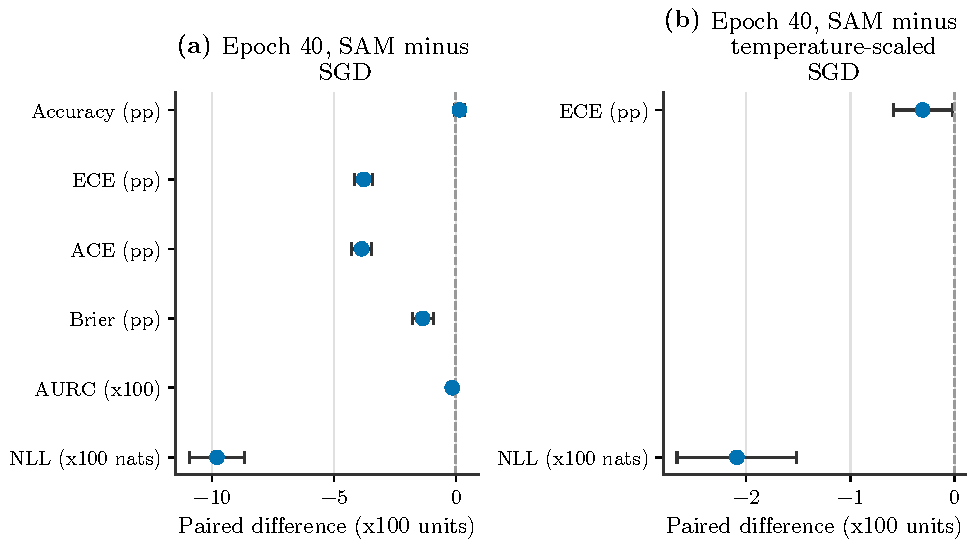
\includegraphics[width=\linewidth,height=0.45\textheight,keepaspectratio]{figures/fig1_v0.pdf}
  \caption{Paired differences, SAM minus the baseline, at epoch 40 over five seeds, in x100 metric units. Points are mean differences and bars are 95\% t-intervals (df = 4): percentage points for accuracy, ECE, ACE, Brier and AURC, and x100 NLL units for NLL. Left: against SGD. Right: against temperature-scaled SGD. The accuracy interval includes zero, and the NLL gap against temperature-scaled SGD excludes zero.}
  \label{fig:paired}
\end{figure}

Table~\ref{tab:pairseed} gives the per-seed paired differences for the two main metrics at epoch 40. Each row is one seed, so the variance of the effect shows directly.

\begin{table}[!htbp]
\centering
\footnotesize
\caption{Artifact 1 (Iteration 1). Per-seed paired differences at epoch 40, SAM minus SGD, read from the paired-test records. The sign is the same for every seed on both metrics.}
\label{tab:pairseed}
\begin{tabular}{rrr}
\toprule
Seed & ECE difference & NLL difference \\
\midrule
0 & -0.03631 & -0.09233 \\
1 & -0.04284 & -0.11242 \\
2 & -0.03537 & -0.09602 \\
3 & -0.03670 & -0.08911 \\
4 & -0.03770 & -0.09991 \\
\bottomrule
\end{tabular}
\end{table}

\paragraph{Training length.} The artifact tested whether the ECE advantage grows with training length by comparing the SGD-minus-SAM ECE advantage at three lengths: the 5-epoch compressed schedule, the 15-epoch compressed schedule and the 40-epoch run. Table~\ref{tab:trainlen} gives those advantages. A positive value means SGD is worse than SAM.

\begin{table}[!htbp]
\centering
\footnotesize
\caption{Artifact 1 (Iteration 1). SGD-minus-SAM ECE advantage by training length, mean over five seeds, from the per-seed values of the compressed and 40-epoch schedules. Positive means SAM is better. The 5-epoch row is a compressed schedule, not an early stop of the 40-epoch run.}
\label{tab:trainlen}
\begin{tabular}{lr}
\toprule
Training length & Mean advantage (SGD minus SAM ECE) \\
\midrule
5 epochs (compressed) & -0.0057 \\
15 epochs (compressed) & +0.0132 \\
40 epochs & +0.0378 \\
\bottomrule
\end{tabular}
\end{table}

The growth from 5 to 40 epochs is significant in the artifact's paired test (difference 0.0435, 95\% CI [0.0376, 0.0494]). The 5-epoch row is negative, so at the 5-epoch schedule SAM's ECE is higher than SGD's. That reverses the early-stopping prediction in criterion (c) of the hypothesis, and the record shows it as a reversal. The reversal is small in NLL terms but present in ECE, with SAM's compressed-5 ECE at 0.0149 against SGD's 0.0092. The compressed schedules are separate training runs, so this reversal is a comparison across schedules and not along one trajectory. The within-run reading is given in Iteration 2 (Table~\ref{tab:gap}).

\paragraph{Check.} The artifact computed again the main paired differences and intervals from the saved test logits with separate code, and its control checks did not reject. Table~\ref{tab:check1} reproduces the independent computation, read from its check output. The artifact did not compute again the ECE binning loop or the ACE, Brier and AURC values for every run, and it did not retrain the model. Scope, clarified in Iteration 2: the check covers the primary paired contrasts and the two control checks only.

\begin{table}[!htbp]
\centering
\footnotesize
\caption{Artifact 1 (Iteration 1). Independent computation of the main contrasts from saved test logits, epoch 40. The SciPy and independent intervals agree to the reported digits. Table label corrected in Iteration 2.}
\label{tab:check1}
\begin{tabular}{lrl}
\toprule
Contrast & Mean difference & 95\% CI (manual check) \\
\midrule
Accuracy, SAM minus SGD & +0.00146 & [-0.00071, +0.00363] \\
ECE, SAM minus SGD & -0.03779 & [-0.04145, -0.03412] \\
NLL, SAM minus SGD & -0.09796 & [-0.10918, -0.08673] \\
AURC, SAM minus SGD & -0.00152 & [-0.00212, -0.00092] \\
NLL, SAM minus TS-SGD & -0.02088 & [-0.02662, -0.01514] \\
ECE, SAM minus TS-SGD & -0.00307 & [-0.00590, -0.00024] \\
\bottomrule
\end{tabular}
\end{table}

Control checks: comparing SGD with itself gives a mean ECE difference of exactly 0, and shuffling the test labels gives an accuracy difference of -0.00036 with a 95\% interval of [-0.00235, +0.00163] that includes zero.


This artifact, \path{gen_art_experiment_1}, is the controlled comparison of Iteration 1. Its declared output files are \path{method.py}, \path{full_method_out.json}, \path{mini_method_out.json}, \path{preview_method_out.json} and \path{reproducibility.md}; its per-run values, tuning table and re-derivation record are in \path{results/}. The tables below are read from its re-derivation record and placebo checks.

\begin{table}[!htbp]
\centering
\scriptsize
\caption{Artifact 1 (Iteration 1), gen\_art\_experiment\_1. Independent re-derivation of the headline paired contrasts from saved test logits, epoch 40, five seeds, read from \texttt{results/audit\_rederivation.json}. The scipy and manual intervals are the two computations the record compares.}
\label{tab:audit1}
\begin{tabular}{lrrrr}
\toprule
Contrast & Mean difference & 95\% CI (scipy) & p (scipy) & 95\% CI (manual check) \\
\midrule
Accuracy, SAM minus SGD & +0.00146 & [-0.00071, +0.00363] & 0.1348 & [-0.00071, +0.00363] \\
ECE, SAM minus SGD & -0.03779 & [-0.04145, -0.03412] & 8.825e-06 & [-0.04145, -0.03412] \\
NLL, SAM minus SGD & -0.09796 & [-0.10918, -0.08673] & 1.721e-05 & [-0.10918, -0.08673] \\
AURC, SAM minus SGD & -0.00152 & [-0.00212, -0.00092] & 0.002118 & [-0.00212, -0.00092] \\
NLL, SAM minus TS-SGD & -0.02088 & [-0.02662, -0.01514] & 0.0005405 & [-0.02662, -0.01514] \\
ECE, SAM minus TS-SGD & -0.00307 & [-0.00590, -0.00024] & 0.03962 & [-0.00590, -0.00024] \\
\bottomrule
\end{tabular}
\end{table}
\begin{table}[!htbp]
\centering
\footnotesize
\caption{Artifact 1 (Iteration 1), gen\_art\_experiment\_1. Control checks from the same re-derivation record. The first control compares SGD with itself; the second shuffles the test labels.}
\label{tab:placebo1}
\begin{tabular}{p{3.6cm}rlrp{4.8cm}}
\toprule
Control & Mean difference & 95\% CI (scipy) & p (scipy) & Expected result \\
\midrule
SGD minus SGD, ECE & +0.00000 & n/a & n/a & mean 0, test must not reject (p nan or 1) \\
Accuracy, shuffled test labels & -0.00036 & [-0.00235, +0.00163] & 0.6412 & CI includes zero (test must not reject) \\
\bottomrule
\end{tabular}
\end{table}
\paragraph{Pooled reliability bins.} The artifact's \texttt{results/reliability\_bins\_pooled.json} gives the test-set reliability bins for SGD, temperature-scaled SGD and SAM. Table~\ref{tab:reliabA} and Table~\ref{tab:reliabB} give them with counts, mean confidence and accuracy per bin. The shape of the epoch-40 gap is shown in the bins. Raw SGD places 43,961 of its 50,000 pooled predictions in the top bin (0.933 to 1.000), where its mean confidence is 0.9965 and its accuracy is 0.9669, so its confidence exceeds its accuracy there by about 0.030. SAM places 37,493 predictions in that bin, with a mean confidence of 0.9922 and an accuracy of 0.9903, a gap of about 0.002. Temperature-scaled SGD places 37,858 predictions there, with a mean confidence of 0.9905 and an accuracy of 0.9865. The raw ECE advantage of SAM is therefore concentrated in the top bin: SAM is better matched there, and it places fewer predictions in that bin. This table was not in the Iteration 1 report; it is reported here as a re-read of an Iteration 1 output.

\begin{table}[!htbp]
\centering
\footnotesize
\caption{Artifact 1 (Iteration 1). Pooled test-set reliability bins for SGD and temperature-scaled SGD, 50,000 predictions each (five seeds of 10,000 test images). Read from \texttt{results/reliability\_bins\_pooled.json}. The same bins for SAM are in the next table.}
\label{tab:reliabA}
\begin{tabular}{lrrrrrr}
\toprule
Bin & SGD n & SGD conf. & SGD acc. & TS-SGD n & TS conf. & TS acc. \\
\midrule
0.000 to 0.067 & 0 & n/a & n/a & 0 & n/a & n/a \\
0.067 to 0.133 & 0 & n/a & n/a & 0 & n/a & n/a \\
0.133 to 0.200 & 0 & n/a & n/a & 0 & n/a & n/a \\
0.200 to 0.267 & 0 & n/a & n/a & 11 & 0.2414 & 0.3636 \\
0.267 to 0.333 & 12 & 0.3080 & 0.2500 & 67 & 0.3092 & 0.2388 \\
0.333 to 0.400 & 36 & 0.3730 & 0.2778 & 183 & 0.3746 & 0.3552 \\
0.400 to 0.467 & 99 & 0.4385 & 0.3333 & 410 & 0.4358 & 0.4488 \\
0.467 to 0.533 & 444 & 0.5089 & 0.4505 & 942 & 0.5045 & 0.4841 \\
0.533 to 0.600 & 620 & 0.5672 & 0.5032 & 1143 & 0.5663 & 0.5687 \\
0.600 to 0.667 & 611 & 0.6338 & 0.4828 & 1163 & 0.6334 & 0.6019 \\
0.667 to 0.733 & 711 & 0.7011 & 0.5570 & 1300 & 0.7012 & 0.7085 \\
0.733 to 0.800 & 841 & 0.7672 & 0.5981 & 1484 & 0.7682 & 0.7446 \\
0.800 to 0.867 & 1054 & 0.8349 & 0.6603 & 2027 & 0.8359 & 0.8254 \\
0.867 to 0.933 & 1611 & 0.9024 & 0.7151 & 3412 & 0.9037 & 0.8757 \\
0.933 to 1.000 & 43961 & 0.9965 & 0.9669 & 37858 & 0.9905 & 0.9865 \\
\bottomrule
\end{tabular}
\end{table}

\begin{table}[!htbp]
\centering
\footnotesize
\caption{Artifact 1 (Iteration 1). Pooled test-set reliability bins for SAM, the same 50,000 predictions as the previous table. Read from \texttt{results/reliability\_bins\_pooled.json}.}
\label{tab:reliabB}
\begin{tabular}{lrrr}
\toprule
Bin & SAM count & SAM confidence & SAM accuracy \\
\midrule
0.000 to 0.067 & 0 & n/a & n/a \\
0.067 to 0.133 & 0 & n/a & n/a \\
0.133 to 0.200 & 1 & 0.1971 & 0.0000 \\
0.200 to 0.267 & 10 & 0.2444 & 0.1000 \\
0.267 to 0.333 & 71 & 0.3086 & 0.1972 \\
0.333 to 0.400 & 194 & 0.3723 & 0.3505 \\
0.400 to 0.467 & 390 & 0.4379 & 0.4077 \\
0.467 to 0.533 & 1016 & 0.5046 & 0.4970 \\
0.533 to 0.600 & 1254 & 0.5665 & 0.5654 \\
0.600 to 0.667 & 1248 & 0.6330 & 0.6250 \\
0.667 to 0.733 & 1377 & 0.7011 & 0.7066 \\
0.733 to 0.800 & 1637 & 0.7676 & 0.7648 \\
0.800 to 0.867 & 2111 & 0.8354 & 0.8153 \\
0.867 to 0.933 & 3198 & 0.9033 & 0.8971 \\
0.933 to 1.000 & 37493 & 0.9922 & 0.9903 \\
\bottomrule
\end{tabular}
\end{table}

\paragraph{Reading of Artifact 1.} Criterion (a) holds for ECE and NLL with intervals well clear of zero. The accuracy result is no significant difference, with a point estimate of +0.15 percentage points and an interval that crosses zero. Criterion (b) holds for NLL: SAM's NLL is lower than temperature-scaled SGD's by 0.021 with an interval excluding zero, and the Holm p is 0.0027. For ECE the advantage over temperature-scaled SGD is 0.003 with an interval just excluding zero, and it is not significant after Holm correction (p = 0.079). The shift that temperature scaling removes is therefore most of the ECE gap but not all of the NLL gap. Criterion (c) holds in the direction of the hypothesis at 15 and 40 epochs and reverses at 5 epochs.

Two caveats limit how far these results apply. First, SAM is under-fit at epoch 40, so part of its calibration advantage may come from a less-fitted model. Second, the selected learning rate lies at the lower edge of the grid, so a lower learning rate might change the SGD baseline. The second experiment artifact addresses the first caveat directly.

\subsection{Artifact 2: mechanism study at fixed setting}

\paragraph{Setup.} The second artifact uses the same network family, with a 10,000-image validation split and the standard test set. Both optimisers share the initialisation and data order for each seed. The setting was fixed before the runs: learning rate 0.03, momentum 0.9, weight decay 5e-4, batch 128, 60 epochs, cosine schedule, SAM radius 0.1. The learning rate was not tuned for this artifact. That choice differs from Artifact 1, and it means the two artifacts do not share a baseline. The artifact reports summary statistics only at n = 3 seed pairs, with no p-values, so no test can be significant at the conventional level.

\paragraph{Test metrics at epochs 5 and 60.} Table~\ref{tab:perseedA} and Table~\ref{tab:perseedB} give the test metrics for each seed at the two evaluated epochs, read from the artifact's average table. The table is split in two to keep it within the text width.

\begin{table}[!htbp]
\centering
\footnotesize
\caption{Artifact 2 (Iteration 1). Test-set metrics per seed at epochs 5 and 60, read from \texttt{results/method\_out.json}. Accuracy is a fraction. This table gives the test metrics; validation metrics are in the next table.}
\label{tab:perseedA}
\begin{tabular}{llrrrrrr}
\toprule
Optimiser & Seed & Epoch & Test accuracy & Test ECE & Test NLL & Test Brier & Test ACE \\
\midrule
SGD & 0 & 5 & 0.9088 & 0.0105 & 0.2541 & 0.1321 & 0.0090 \\
SGD & 1 & 5 & 0.8978 & 0.0143 & 0.2754 & 0.1472 & 0.0128 \\
SGD & 2 & 5 & 0.8986 & 0.0239 & 0.2791 & 0.1459 & 0.0238 \\
SGD & 0 & 60 & 0.9226 & 0.0466 & 0.3186 & 0.1239 & 0.0466 \\
SGD & 1 & 60 & 0.9239 & 0.0439 & 0.3162 & 0.1246 & 0.0438 \\
SGD & 2 & 60 & 0.9251 & 0.0432 & 0.3105 & 0.1222 & 0.0432 \\
SAM & 0 & 5 & 0.9048 & 0.0167 & 0.2682 & 0.1389 & 0.0170 \\
SAM & 1 & 5 & 0.9054 & 0.0067 & 0.2589 & 0.1361 & 0.0072 \\
SAM & 2 & 5 & 0.8987 & 0.0128 & 0.2746 & 0.1444 & 0.0120 \\
SAM & 0 & 60 & 0.9256 & 0.0282 & 0.2405 & 0.1131 & 0.0282 \\
SAM & 1 & 60 & 0.9233 & 0.0284 & 0.2350 & 0.1131 & 0.0284 \\
SAM & 2 & 60 & 0.9263 & 0.0258 & 0.2415 & 0.1142 & 0.0240 \\
\bottomrule
\end{tabular}
\end{table}

\begin{table}[!htbp]
\centering
\footnotesize
\caption{Artifact 2 (Iteration 1). Validation-split metrics per seed at epochs 5 and 60, same runs as the previous table, read from \texttt{results/method\_out.json}. ECE uses 15 equal-width bins.}
\label{tab:perseedB}
\begin{tabular}{llrrr}
\toprule
Optimiser & Seed & Epoch & Validation ECE & Validation NLL \\
\midrule
SGD & 0 & 5 & 0.0064 & 0.2262 \\
SGD & 1 & 5 & 0.0116 & 0.2559 \\
SGD & 2 & 5 & 0.0179 & 0.2581 \\
SGD & 0 & 60 & 0.0452 & 0.2901 \\
SGD & 1 & 60 & 0.0419 & 0.2803 \\
SGD & 2 & 60 & 0.0429 & 0.2883 \\
SAM & 0 & 5 & 0.0222 & 0.2427 \\
SAM & 1 & 5 & 0.0105 & 0.2412 \\
SAM & 2 & 5 & 0.0098 & 0.2541 \\
SAM & 0 & 60 & 0.0249 & 0.2111 \\
SAM & 1 & 60 & 0.0256 & 0.2224 \\
SAM & 2 & 60 & 0.0236 & 0.2181 \\
\bottomrule
\end{tabular}
\end{table}

At epoch 60 the per-seed paired differences in test ECE (SAM minus SGD) are -0.0184, -0.0155 and -0.0174, all negative. The test NLL differences are -0.0781, -0.0812 and -0.0690, also all negative. The test accuracy differences are +0.0030, -0.0006 and +0.0012, which have mixed signs. At epoch 5 the test ECE differences have no consistent sign.

\paragraph{Temperature scaling.} Table~\ref{tab:tsA2} gives the temperature-scaled values for each seed. The temperature for each model was fitted on the validation split. Scaling changes no predicted class, so accuracy is unchanged by design.

\begin{table}[!htbp]
\centering
\footnotesize
\caption{Artifact 2 (Iteration 1). Temperature-scaled test metrics per seed, read from the artifact's temperature-scaling record. T is the fitted temperature, and the unscaled columns reproduce the test ECE and NLL from the per-seed test table for comparison. Fitted temperatures for SGD at epoch 60 lie near 1.9, and for SAM near 1.4.}
\label{tab:tsA2}
\begin{tabular}{llrrrrr}
\toprule
Optimiser, seed & Epoch & T & Test ECE, scaled & Test ECE, unscaled & Test NLL, scaled & Test NLL, unscaled \\
\midrule
SGD, seed 0 & 5 & 1.0161 & 0.0094 & 0.0105 & 0.2537 & 0.2541 \\
SGD, seed 1 & 5 & 1.0464 & 0.0110 & 0.0143 & 0.2744 & 0.2754 \\
SGD, seed 2 & 5 & 1.1326 & 0.0118 & 0.0239 & 0.2743 & 0.2791 \\
SGD, seed 0 & 60 & 1.8979 & 0.0088 & 0.0466 & 0.2364 & 0.3186 \\
SGD, seed 1 & 60 & 1.8546 & 0.0104 & 0.0439 & 0.2373 & 0.3162 \\
SGD, seed 2 & 60 & 1.8936 & 0.0091 & 0.0432 & 0.2330 & 0.3105 \\
SAM, seed 0 & 5 & 0.8015 & 0.0140 & 0.0167 & 0.2651 & 0.2682 \\
SAM, seed 1 & 5 & 0.9085 & 0.0074 & 0.0067 & 0.2587 & 0.2589 \\
SAM, seed 2 & 5 & 1.0211 & 0.0123 & 0.0128 & 0.2743 & 0.2746 \\
SAM, seed 0 & 60 & 1.3787 & 0.0070 & 0.0282 & 0.2190 & 0.2405 \\
SAM, seed 1 & 60 & 1.3947 & 0.0052 & 0.0284 & 0.2160 & 0.2350 \\
SAM, seed 2 & 60 & 1.3556 & 0.0089 & 0.0258 & 0.2224 & 0.2415 \\
\bottomrule
\end{tabular}
\end{table}

Averaged over seeds at epoch 60, scaling moves SGD's test ECE from 0.0446 to 0.0094 and SAM's from 0.0275 to 0.0070. The SGD model's fitted temperature is well above 1, which matches its overconfidence. The SAM model's fitted temperature is also above 1 at epoch 60, so SAM is still overconfident, but less so. Averaged over seeds, scaling moves SGD's test NLL from 0.3151 to 0.2356 and SAM's from 0.2390 to 0.2192. The SAM advantage in NLL therefore decreases from 0.076 to 0.016 NLL units after scaling. Most of the unscaled NLL gap is a global confidence shift, and a residual remains.

\begin{figure}[!htbp]
  \centering
  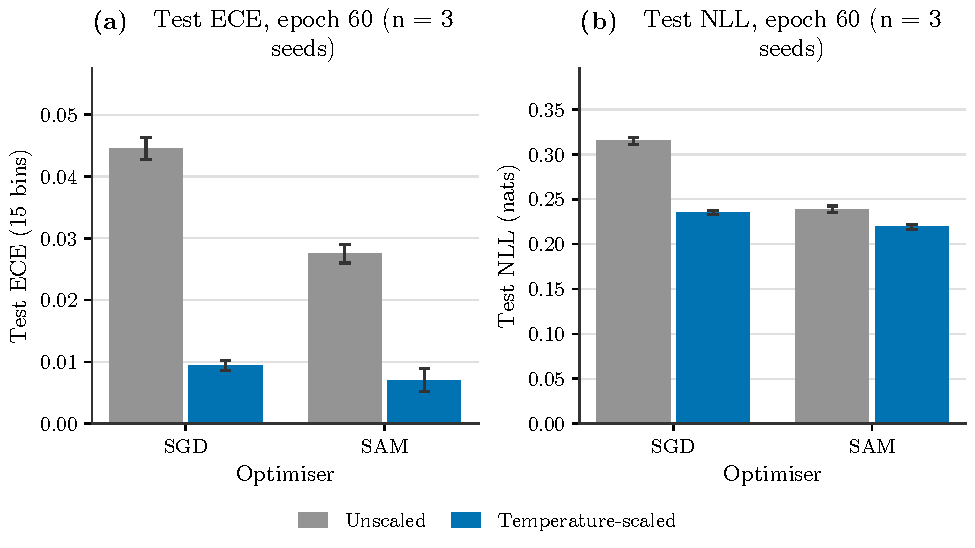
\includegraphics[width=\linewidth,height=0.45\textheight,keepaspectratio]{figures/fig2_v0.pdf}
  \caption{Test ECE (a) and test NLL (b) at epoch 60 for SGD and SAM, unscaled and temperature-scaled. Bars are means over three seeds and error bars are sample standard deviations across seeds. After temperature scaling, the SGD and SAM ECE values are close, and the SAM NLL advantage remains.}
  \label{fig:epoch60}
\end{figure}

\paragraph{Training loss and calibration over training.} Table~\ref{tab:perepoch} gives the per-epoch means at selected epochs, averaged over the three seeds, read from the per-epoch record. The evaluation grid is every epoch from 1 to 60; the rows shown are a subset of it. The top Hessian eigenvalue is estimated by 20 power iterations on a fixed 2,000-image batch. The SAM loss increase within the radius is in the same record and is reported at every logged epoch in Table~\ref{tab:hessian} (Iteration 2).

\begin{table}[!htbp]
\centering
\footnotesize
\caption{Artifact 2 (Iteration 1). Per-epoch means over three seeds at selected epochs, read from \texttt{results/per\_epoch.json}. Training loss is the mean over the epoch. Validation ECE is the mean of the three seeds. Top Hessian eigenvalue is the mean of the three seeds at evaluated epochs.}
\label{tab:perepoch}
\begin{tabular}{rrrrrrr}
\toprule
Epoch & SGD loss & SGD val.\ ECE & SGD Hessian & SAM loss & SAM val.\ ECE & SAM Hessian \\
\midrule
1 & 0.4662 & 0.0160 & 24.95 & 0.5477 & 0.0116 & 9.18 \\
2 & 0.2873 & 0.0106 & 20.69 & 0.3167 & 0.0144 & 6.80 \\
5 & 0.1996 & 0.0119 & 19.09 & 0.2256 & 0.0141 & 6.21 \\
10 & 0.1314 & 0.0219 & 15.72 & 0.1724 & 0.0094 & 6.60 \\
15 & 0.0925 & 0.0313 & 20.58 & 0.1399 & 0.0064 & 6.33 \\
20 & 0.0610 & 0.0368 & 19.19 & 0.1131 & 0.0092 & 6.94 \\
30 & 0.0188 & 0.0457 & 25.02 & 0.0751 & 0.0136 & 8.01 \\
40 & 0.0050 & 0.0440 & 14.55 & 0.0486 & 0.0180 & 7.50 \\
50 & 0.0046 & 0.0434 & 19.89 & 0.0343 & 0.0243 & 7.43 \\
60 & 0.0045 & 0.0433 & 20.20 & 0.0306 & 0.0247 & 7.13 \\
\bottomrule
\end{tabular}
\end{table}

Correction (Iteration 2): the SGD top Hessian eigenvalue is between 1.9 and 3.35 times the SAM value across the logged epochs (2.7 at epoch 1, 3.35 at epoch 25, 1.9 at epoch 40). The earlier claim, two to three times at every evaluated epoch, was too broad. The ratio at each logged epoch is in Table~\ref{tab:hessian}. SGD's validation ECE rises from 0.012 at epoch 5 to 0.043 at epoch 60, while its training loss falls to 0.005. SAM's validation ECE falls to a minimum of 0.0064 at epoch 15 and then rises to 0.025 at epoch 60, while its training loss stays near 0.03. Both optimisers become less calibrated as training continues past the point where their validation ECE is lowest, and the rise in SGD's validation ECE is larger. The per-epoch means do not show a gap at epoch 5, which matches the sign-mixed comparison in the per-seed test table.

\paragraph{Matched training loss.} The artifact compared the two optimisers at equal training loss, by interpolating each run's per-epoch values on a common grid of eight training-loss levels. Table~\ref{tab:matchA} gives the per-seed means of the differences over that grid. A negative value means SAM is lower.

\begin{table}[!htbp]
\centering
\footnotesize
\caption{Artifact 2 (Iteration 1). Matched training-loss comparison, SAM minus SGD, per seed, averaged over the eight-level grid. Read from the matched-loss record in \texttt{results/method\_out.json}.}
\label{tab:matchA}
\begin{tabular}{rrr}
\toprule
Seed & Mean top Hessian eigenvalue difference & Mean validation ECE difference \\
\midrule
0 & -15.62 & -0.0108 \\
1 & -13.34 & -0.0096 \\
2 & -12.16 & -0.0141 \\
Mean & -13.71 & -0.0115 \\
\bottomrule
\end{tabular}
\end{table}

At matched training loss, SAM's top Hessian eigenvalue is about 12 to 16 lower, and its validation ECE is about 0.010 to 0.014 lower. The grid for seed 0 shows that the validation ECE gap is largest at the lower training losses and decreases to about zero, and for some levels reverses sign, at the highest training losses. The matched comparison therefore does not show the gap is constant across training losses.

\paragraph{Statistics for Artifact 2.} Table~\ref{tab:stats2} gives the per-seed contrasts at epoch 60 and at epoch 5 read from the artifact's statistics record. The artifact reports no p-values, and the signs are the evidence.

\begin{table}[!htbp]
\centering
\footnotesize
\caption{Artifact 2 (Iteration 1). SAM minus SGD per seed, read from the artifact's statistics record. Sign pattern is written in seed order, ``-'' for negative, ``+'' for positive.}
\label{tab:stats2}
\begin{tabular}{lrrrrl}
\toprule
Metric & Seed 0 & Seed 1 & Seed 2 & Mean & Sign pattern \\
\midrule
Test ECE, epoch 60 & -0.0184 & -0.0155 & -0.0174 & -0.0171 & --- \\
Test NLL, epoch 60 & -0.0781 & -0.0812 & -0.0690 & -0.0761 & --- \\
Test accuracy, epoch 60 & +0.0030 & -0.0006 & +0.0012 & +0.0012 & +-+ \\
Validation ECE, epoch 5 & +0.0158 & -0.0011 & -0.0081 & +0.0022 & +-- \\
\bottomrule
\end{tabular}
\end{table}

The Hessian sign check found no negative top eigenvalue in any of the 84 checkpoints, so the power iteration returned the dominant curvature in each case.


This artifact, \path{gen_art_experiment_2}, is the mechanism study of Iteration 1, at a fixed learning rate of 0.03 with three seeds per optimiser. Its declared output files are \path{method.py}, \path{full_method_out.json}, \path{mini_method_out.json}, \path{preview_method_out.json} and \path{reproducibility.md}; the per-epoch record, logits, run configuration and run notes are in \path{results/}. Its run notes record the status of each run, below.

\begin{table}[!htbp]
\centering
\footnotesize
\caption{Artifact 2 (Iteration 1), gen\_art\_experiment\_2. Run status from \texttt{results/notes.md}: the last recorded epoch and final status of each optimiser and seed.}
\label{tab:runs2}
\begin{tabular}{llrl}
\toprule
Run & Last recorded epoch & Final status \\
\midrule
sgd seed0 & 60 & ok \\
sgd seed1 & 60 & ok \\
sgd seed2 & 60 & ok \\
sam seed0 & 60 & ok \\
sam seed1 & 60 & ok \\
sam seed2 & 60 & ok \\
\bottomrule
\end{tabular}
\end{table}

The run notes also record the top Hessian eigenvalue sign check: it is negative at 0 of 84 checkpoints, so the power iteration returned the dominant curvature in each case. The per-epoch and matched-loss tables for this artifact are those already reported above.

\subsection{Prior-work check (research artifact)}\label{sec:prior}

The third direction set in Iteration 1 was a check of prior work, designed to find which published work runs SAM against temperature-scaled SGD on a small network, which baselines and radius ranges are expected, and which metric definitions to use. It was run as a research artifact, and it produced a completed report with a verdict. The earlier draft of this record said that this check did not run; that statement is withdrawn. The check produced \texttt{research\_report.md} and \texttt{research\_out.json}, and its verification file records one passage that could not be matched to the fetched source text (detailed below).

The artifact read the primary texts of five papers in full, through PDF text extraction, and read one further paper at its abstract page. Its verdict on novelty is ``partly done''. Tan et al.\ report, for ResNet-56 on CIFAR-10 and CIFAR-100, that the ECE of SGD is ``approximately six times larger than the ECE of SAM'', and that ``the uncalibrated ECE of SAM is generally smaller than the calibrated ECE of SGD by calibration methods such as temperature scaling'' \citep{tan2026}. Those are the settings the artifact checked against the source text. Nothing in the read sources covers a small CNN, Fashion-MNIST, or NLL and Brier as metrics. Foret et al.\ establish SAM on Fashion-MNIST for accuracy only. Nixon et al.\ are a source of calibration metrics, not a SAM study. The verdict rests on search coverage, not an exhaustive review, and a paper published after the search date could be missed.

Table~\ref{tab:research} gives the artifact's comparison of the sources. Its last column is the artifact's own reading of each source for the SAM-versus-temperature-scaling question.

\begin{table}[!htbp]
\centering
\footnotesize
\caption{Research artifact (Iteration 1), prior-work comparison, read from \texttt{research\_report.md}, section 2. Source names are as the artifact gives them, without its own numbering. The artifact's rho and learning-rate protocol column is omitted here for width; it is in \texttt{research\_report.md}, section 2.}
\label{tab:research}
\begin{tabularx}{\linewidth}{>{\raggedright\arraybackslash}p{2.2cm}>{\raggedright\arraybackslash}p{3.0cm}>{\raggedright\arraybackslash}p{2.4cm}>{\raggedright\arraybackslash}X>{\raggedright\arraybackslash}p{2.6cm}>{\raggedright\arraybackslash}p{2.6cm}}
\toprule
Source & Setting & Optimiser & Metrics reported & Temperature scaling as control & Verdict for the SAM-vs-TS question \\
\midrule
Tan et al. 2026 & ResNet-20/56, ResNeXt-29, WRN-28-10, PyramidNet-110 on CIFAR-10/100; ResNet-18 for OOD; ImageNet-1K per abstract & SGD (momentum 0.9, cosine) vs SAM; CSAM proposed & Test accuracy, ECE, ClasswiseECE, AdaECE, TCE, AUROC; mean and std over 3 seeds; no NLL or Brier in the excerpts read & Yes: TS and isotonic regression applied to SGD and to SAM & Closest prior work. Compares SAM with SGD plus TS, but not on a small CNN, not on Fashion-MNIST, and not with NLL or Brier. \\
Morosini et al. 2026 & ``small vision tasks'', multiple gradient methods (GD, SGD, AdamW, Muon, SAM) & Several, SAM included & ECE, KCE, and a curvature (Gauss-Newton) sharpness proxy & Not evident in the excerpts read & Related: studies calibration as a training-time phenomenon; does not compare SAM against temperature-scaled SGD. \\
Nixon et al. 2019 & Calibration-measure study on MNIST, Fashion-MNIST, CIFAR-10/100, ImageNet & Recalibration methods (including temperature scaling) applied after training & ECE, SCE, ACE, and others & Yes, as a recalibration method being ranked & Metric source, not a SAM comparison. Shows that the ranking of recalibrators depends on the metric chosen. \\
Foret et al. 2021 & WRN-28-10 on Fashion-MNIST, CIFAR-10/100, SVHN, ImageNet & SGD vs SAM & Test error only; no calibration metric found in the grep output & No & Establishes SAM on Fashion-MNIST for accuracy only. Not a calibration study. \\
M\"uller et al. 2019 & Label smoothing for multi-class networks & Label smoothing (reference baseline) & Abstract only read & Not read & Baseline reference only; the abstract says label smoothing prevents over-confidence. \\
\bottomrule
\end{tabularx}
\end{table}

The artifact also lists what it could not verify. The Fashion-MNIST value of rho for SAM in a calibration setting was not found. Foret et al.'s Fashion-MNIST radius is not stated in the main text, and its appendix C.1 was not read. A web page reporting that SAM and calibration relate through sharper minima was seen only as a search snippet and is not used. The verification file (\texttt{research\_verification.json}) records \texttt{valid: false}: one quoted passage attributed to a Nixon et al.\ source could not be found in the fetched text. The passage check did not find any other failed quote, and the artifact's conclusions do not rest on that one quote, but the quote itself is unconfirmed and is not reproduced here.

\subsection{What Iteration 1 established}

On the controlled comparison, SAM at a validation-selected learning rate and radius has a lower test ECE and a lower test NLL than SGD, with paired intervals excluding zero and a consistent sign across all five seeds. Its test accuracy is the same within the seed variance. The NLL advantage remains against temperature-scaled SGD, with Holm p = 0.0027. The ECE advantage over the same baseline is small and not significant after correction.

On the mechanism study, the ECE and NLL differences at epoch 60 keep their sign across three seeds, and the matched-loss comparison finds a lower top Hessian eigenvalue and a lower validation ECE for SAM. Temperature scaling removes most of the test ECE and NLL gap at epoch 60, and what remains of the NLL gap is about one-fifth of the unscaled gap.

Against the hypothesis:

\begin{enumerate}
\item Criterion (a), lower test ECE and NLL than tuned SGD: supported by Artifact 1 with five seeds, and by Artifact 2 as summary statistics at three seeds.
\item Criterion (b), NLL advantage after temperature scaling: supported by Artifact 1 (Holm p = 0.0027). Artifact 2 shows a residual scaled NLL advantage of 0.016 NLL units on average, without a test.
\item Criterion (c), gap larger at full training than at short training: supported at 15 and 40 epochs in Artifact 1 under compressed schedules. Reversed at 5 epochs under compressed training, where SAM's ECE is higher. Artifact 2 shows no consistent sign at epoch 5.
\item Accuracy: no significant difference in either artifact, recorded as such.
\end{enumerate}

Two caveats apply to every reading. SAM is less fitted than SGD at the end of both main schedules, so the calibration advantage may in part reflect a less-fitted model; the matched-loss comparison in Artifact 2 addresses this only at the training losses the runs reached. And the two artifacts use different learning rates, one tuned and one fixed, so their numbers are not comparable.

\subsection{Failed directions and dropped work}

\begin{enumerate}
\item SAM at learning rate 0.03 with radius 0.2 failed to train (training loss 2.302, validation accuracy 0.1305) and was excluded from selection. This is a failed setting, not a finding about SAM's calibration.
\item The 60-epoch extension of Artifact 1 was not run. The artifact reports that SAM is under-fit at epoch 40 and that this extension would test it. The question stays open.
\item The early-stopping test of criterion (c) was replaced by compressed schedules, which are separate full training runs. The record keeps this change. The 40-epoch run's own epoch 5 and epoch 15 values are in Table~\ref{tab:gap} (Iteration 2) and differ from the compressed runs at the same epoch count.
\end{enumerate}

\subsection{Review of Iteration 1 and hypothesis update}

The Iteration 1 review scored the record 4 of 5 and did not block it. The reviewer recomputed the headline paired contrasts from the per-run file and found them to match, and recorded these as major points: (1) the calibrated ECE comparison was not like-for-like, because Table~\ref{tab:paired}'s ``SAM minus TS-SGD'' row compares uncalibrated SAM with calibrated SGD, and the record still claimed a small calibrated ECE advantage; (2) the record had no nearest-neighbour comparison with Tan et al.\ and Morosini et al., and the planned prior-work check had not run; (3) criterion (a) was stated as holding without being scoped to the fit gap and to the grid-edge learning rates; (4) criterion (c) rested on separately trained compressed schedules, not on one training trajectory; (5) the reasoning for the design choices was thin, and the pooled reliability bins and Artifact 2's rho-ball loss increase were on disk but not reported.

The hypothesis update moved the run by deepening it, not by pivoting. The update kept the NLL lead, which survived temperature scaling, and named its two open threats as the fit confound and the grid-edge tuning. The reviewer's first point is taken up in Iteration 2 by a like-for-like temperature-scaled comparison, the second by the prior-work artifact above and by Iteration 2's review, the third and fourth by the matched-loss and within-run analyses in Iteration 2, and the fifth by the re-reads in this section.

\section{Iteration 2}

\subsection{Why this iteration ran what it ran}

The review feedback on the Iteration 1 report had five major points and three further points. Four of them decided what this iteration measured. The first was that the calibrated ECE comparison compared uncalibrated SAM with temperature-scaled SGD, so the paired temperature-scaled comparison was missing. The second was that the primary conclusion on criterion (a) was not scoped to two confounds: the fit gap between the optimisers at epoch 40, and the selected learning rates, which were at the lower edge of the grid. The third was that criterion (c) rested on separately trained compressed schedules, which do not follow one training trajectory. The fourth was that the related-work comparison and the nearest published results were not named in the report. The points were corrections of wording and of one stated ratio.

The hypothesis update kept the NLL claim, dropped the raw ECE claim as a calibration gain, and named the next test: whether the NLL gain holds at matched training loss, and with learning rates away from the grid edge. The update also named the checks in order: two further runs on the Iteration 1 setting, a matched-loss comparison with a temperature-scaled control, and one per-epoch read of a single 40-epoch trajectory.

Three artifacts were run to address those points, and one more was run as a reading of existing outputs. Each design choice is recorded here, because the choice decides what the result can and cannot say.

\begin{enumerate}
\item \textbf{Artifact 3} re-runs the primary comparison with the learning rates tuned on validation NLL over a grid that extends below the previous edge. The Iteration 1 grid for the SGD learning rate was $\{0.01, 0.03, 0.1\}$, and it selected its lower edge. This artifact used 0.0003, 0.001, 0.003, 0.01 and 0.03 for SGD, and 0.001, 0.003, 0.01 and 0.03 for SAM, plus the radius grid, so that the selected values lie inside the grid. It keeps five paired seeds, the Iteration 1 architecture and split, and the same temperature-scaled control, and it reports the final training loss beside every calibration row.
\item \textbf{Artifact 4} matches training loss directly. Artifact 1 showed that SAM ends with a much higher training loss than SGD, so an NLL gap could be a fit gap. This artifact compares SAM at 40 epochs with SGD at the epoch count whose training loss matches SAM's within 0.01. We call the training loss the mean loss on the full training set, computed after the epoch with batch normalisation in inference mode. The matching epoch was chosen on seed 100, and the SGD learning rate was fixed at 0.01 so that only the training length differs between the conditions. The design has a known weakness, stated in its caveats: Artifact 3 found SGD at learning rate 0.01 to be the worst of its five SGD rates on validation NLL, so this baseline is weaker than the one Artifact 3 selected.
\item \textbf{Evaluation 1} reads the training-length trajectory from outputs the run already holds. It trains nothing and computes no logits again. It reports the SAM-minus-SGD gap at each evaluated epoch inside each source, and it keeps the two sources separate. The compressed-schedule comparison of Iteration 1 is replaced by its within-run checkpoints, which are read from the same training run.
\end{enumerate}

Every number in this section was read from the artifacts' output files in this iteration. Where a figure is taken from an artifact's own summary, the text says so.

\subsection{Artifact 3: the primary comparison with learning rates tuned off the grid edge}

\paragraph{Setup.} The network, data split, batch size, momentum, weight decay and cosine schedule are those of Artifact 1. Each condition is trained for 40 epochs. Learning rates and the SAM radius were selected on tuning seed 101 by lowest final validation NLL, and the test set was not used for selection. Table~\ref{tab:tune2} gives the full tuning grid. The selected settings are SGD at learning rate 0.001 and SAM at learning rate 0.01 with radius 0.1. Neither lies on an edge of its grid.

\begin{table}[!htbp]
\centering
\footnotesize
\caption{Artifact 3 (Iteration 2). Tuning grid on seed 101, 40 epochs, final-epoch values, validation NLL. Read from \texttt{results/tuning\_table.csv}. The selection rule is lowest final validation NLL.}
\label{tab:tune2}
\begin{tabular}{llrrrr}
\toprule
Condition & Learning rate & rho & Validation NLL & Validation accuracy & Final training loss \\
\midrule
SGD & 0.0003 & none & 0.24995 & 0.9113 & 0.23453 \\
SGD & 0.001 & none & 0.21415 & 0.9233 & 0.12430 \\
SGD & 0.003 & none & 0.23818 & 0.9258 & 0.03788 \\
SGD & 0.01 & none & 0.27298 & 0.9288 & 0.00871 \\
SGD & 0.03 & none & 0.26651 & 0.9320 & 0.00608 \\
SAM & 0.001 & 0.05 & 0.22085 & 0.9195 & 0.19937 \\
SAM & 0.001 & 0.1 & 0.24760 & 0.9077 & 0.24128 \\
SAM & 0.001 & 0.2 & 0.30157 & 0.8864 & 0.30399 \\
SAM & 0.003 & 0.05 & 0.18776 & 0.9321 & 0.12601 \\
SAM & 0.003 & 0.1 & 0.20577 & 0.9260 & 0.17906 \\
SAM & 0.003 & 0.2 & 0.24244 & 0.9117 & 0.23560 \\
SAM & 0.01 & 0.05 & 0.19161 & 0.9336 & 0.04923 \\
SAM & 0.01 & 0.1 & 0.18244 & 0.9331 & 0.11087 \\
SAM & 0.01 & 0.2 & 0.20774 & 0.9273 & 0.18431 \\
SAM & 0.03 & 0.05 & 0.21143 & 0.9313 & 0.02896 \\
SAM & 0.03 & 0.1 & 0.18722 & 0.9335 & 0.07043 \\
SAM & 0.03 & 0.2 & 0.19445 & 0.9289 & 0.14705 \\
\bottomrule
\end{tabular}
\end{table}

The SGD learning rate that Iteration 1 selected, 0.01, is the fourth of five in this grid, and its validation NLL is 0.273, against 0.214 at 0.001. The Iteration 1 baseline was therefore not the best SGD setting on validation NLL. That is the first finding of this iteration, and it is recorded as a correction to the Iteration 1 reading of the SGD baseline in the corrections section at the end.


This artifact, \path{gen_art_experiment_3}, re-runs the primary comparison with learning rates tuned on validation NLL, over a grid that extends below the Iteration 1 edge. Its declared output files are \path{method.py}, \path{full_method_out.json}, \path{mini_method_out.json}, \path{preview_method_out.json} and \path{reproducibility.md}; the tables, logits, reliability bins and the re-derivation and placebo records are in \path{results/}. The selection record below is the output of that tuning, and the grid it selected from is Table~\ref{tab:tune2}.

\begin{table}[!htbp]
\centering
\footnotesize
\caption{Artifact 3 (Iteration 2), gen\_art\_experiment\_3. Selected settings, read from \texttt{results/selection.json}. Selection criterion: final-epoch validation NLL on the raw logits, lowest wins, tuning seed 101. Neither selection lies on an edge of its grid, and the record marks that an extension run was used.}
\label{tab:select3}
\begin{tabular}{llrr}
\toprule
Condition & Learning rate & rho & Validation NLL (selected) \\
\midrule
SGD & 0.001 & none & 0.21415 \\
SAM & 0.01 & 0.1 & 0.18244 \\
\bottomrule
\end{tabular}
\end{table}

The record's note on this control reads: post hoc, not part of the pre-registered twelve-row family, reported separately, with both temperature-scaled conditions evaluated against a fixed shuffle of the test labels. The rows below are that control.

\begin{table}[!htbp]
\centering
\scriptsize
\caption{Artifact 3 (Iteration 2), gen\_art\_experiment\_3. Post hoc shuffled-label control on the temperature-scaled conditions, SAM minus SGD, both temperature-scaled, five seeds. Read from \texttt{results/posthoc\_placebo\_ts.json}.}
\label{tab:posthoc3}
\begin{tabular}{lrrrr}
\toprule
Metric (shuffled labels) & Mean difference & 95\% CI & p (two-sided) & Holm p \\
\midrule
acc & -0.00032 & [-0.00200, +0.00136] & 0.625 & 0.625 \\
nll & +0.91085 & [+0.72974, +1.09196] & 0.0001527 & 0.0004688 \\
ece & +0.01129 & [+0.00915, +0.01344] & 0.000128 & 0.0004688 \\
brier & +0.01717 & [+0.01588, +0.01846] & 3.169e-06 & 1.584e-05 \\
ace & +0.01127 & [+0.00917, +0.01337] & 0.0001172 & 0.0004688 \\
\bottomrule
\end{tabular}
\end{table}
\begin{table}[!htbp]
\centering
\scriptsize
\caption{Artifact 3 (Iteration 2), gen\_art\_experiment\_3. Independent re-derivation of the headline contrasts and the shuffled-label NLL placebo, read from \texttt{results/audit\_rederivation.json}.}
\label{tab:audit3}
\begin{tabular}{lrrr}
\toprule
Contrast & Mean difference & 95\% CI & p (two-sided) \\
\midrule
SAM minus TS-SGD: NLL & -0.03259 & [-0.03961, -0.02558] & 0.0002085 \\
SAM minus SGD: NLL & -0.03561 & [-0.04275, -0.02848] & 0.0001573 \\
SAM minus TS-SGD: ECE & +0.00204 & [-0.00019, +0.00427] & 0.0643 \\
SAM minus SGD: ECE & -0.00500 & [-0.00786, -0.00213] & 0.008392 \\
NLL, SAM minus SGD, shuffled labels (placebo) & -0.22405 & [-0.35506, -0.09304] & 0.008983 \\
\bottomrule
\end{tabular}
\end{table}
\begin{table}[!htbp]
\centering
\footnotesize
\caption{Artifact 3 (Iteration 2), gen\_art\_experiment\_3. Fitted temperatures per seed on validation logits, read from \texttt{results/audit\_rederivation.json}.}
\label{tab:temps3}
\begin{tabular}{lrr}
\toprule
Seed & T (SGD) & T (SAM) \\
\midrule
1 & 1.0454 & 0.9278 \\
2 & 1.0621 & 0.9528 \\
3 & 1.0565 & 0.9377 \\
4 & 1.0316 & 0.9205 \\
5 & 1.0481 & 0.9502 \\
\bottomrule
\end{tabular}
\end{table}
\paragraph{Paired contrasts.} Table~\ref{tab:primary} gives the twelve-row paired family, with five seeds, paired t-intervals at df = 4, and Holm correction over the family. Figure~\ref{fig:nll} draws the NLL rows and Figure~\ref{fig:ece} the ECE rows.

\begin{table}[!htbp]
\centering
\footnotesize
\caption{Artifact 3 (Iteration 2). Paired differences over five seeds at 40 epochs, SAM minus the baseline, from \texttt{results/analysis\_tables.json}. The family has twelve contrasts; Holm p is over that family. The rows marked TS compare temperature-scaled models. The two rows marked TS-SAM minus TS-SGD are one comparison: their per-seed ECE and NLL differences are identical in the artifact.}
\label{tab:primary}
\begin{tabularx}{\linewidth}{>{\raggedright\arraybackslash}X r l r r c}
\toprule
Contrast & Mean difference & 95\% CI & p (two-sided) & Holm p & Holm, 0.05 \\
\midrule
SAM minus SGD: accuracy & +0.00958 & [+0.00649, +0.01267] & 0.0010 & 0.0070 & yes \\
SAM minus SGD: ECE & -0.00500 & [-0.00786, -0.00213] & 0.0084 & 0.0336 & yes \\
SAM minus SGD: NLL & -0.03561 & [-0.04275, -0.02848] & 0.0002 & 0.0016 & yes \\
SAM minus SGD: Brier & -0.01575 & [-0.01845, -0.01304] & 8.6e-05 & 0.0010 & yes \\
SAM minus SGD: ACE & -0.00598 & [-0.00891, -0.00305] & 0.0048 & 0.0240 & yes \\
SAM minus TS-SGD: accuracy & +0.00958 & [+0.00649, +0.01267] & 0.0010 & 0.0070 & yes \\
SAM minus TS-SGD: ECE & +0.00199 & [-0.00028, +0.00427] & 0.0718 & 0.2154 & no \\
SAM minus TS-SGD: NLL & -0.03259 & [-0.03958, -0.02561] & 0.0002 & 0.0018 & yes \\
SAM minus TS-SGD: Brier & -0.01524 & [-0.01789, -0.01260] & 8.9e-05 & 0.0010 & yes \\
SAM minus TS-SGD: ACE & +0.00128 & [-0.00185, +0.00440] & 0.3208 & 0.3208 & no \\
TS-SAM minus TS-SGD: ECE & +0.00199 & [-0.00028, +0.00427] & 0.0718 & 0.2154 & no \\
TS-SAM minus TS-SGD: NLL & -0.03259 & [-0.03958, -0.02561] & 0.0002 & 0.0018 & yes \\
\bottomrule
\end{tabularx}
\end{table}

\begin{figure}[!htbp]
  \centering
  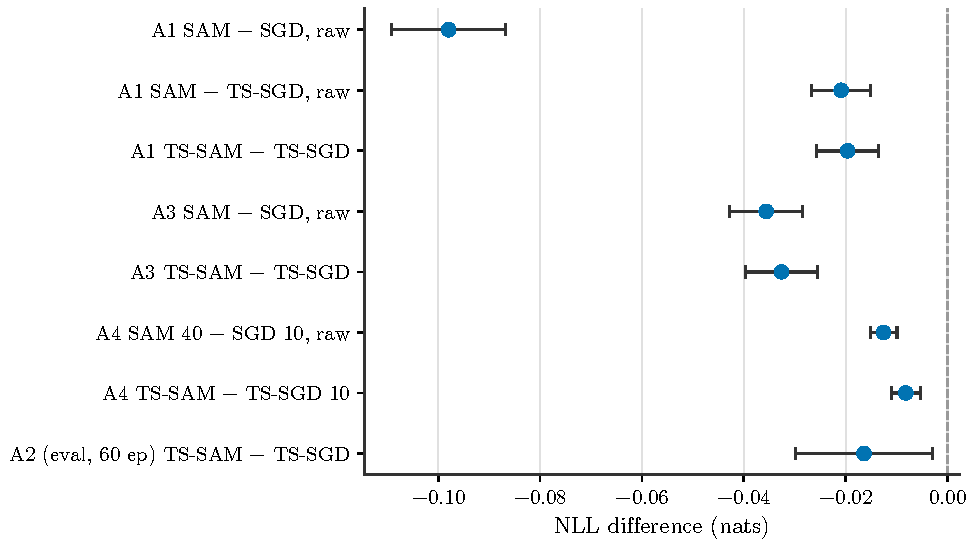
\includegraphics[width=\linewidth,height=0.45\textheight,keepaspectratio]{figures/fig3_v0.pdf}
  \caption{Paired NLL differences (SAM minus comparator) across four artifacts: every interval lies below zero, so SAM's NLL is lower than each comparator, including temperature-scaled SGD (TS). Dots are means; horizontal lines are 95\% t-intervals (df = 4 for five-seed rows, df = 2 for the three-seed Artifact 2 row, which is the evaluation's epoch-60 endpoint). Rows: Artifact 1 (the Iteration 1 controlled comparison), Artifact 3, Artifact 4 and the Artifact 2 evaluation row.}
  \label{fig:nll}
\end{figure}

\begin{figure}[!htbp]
  \centering
  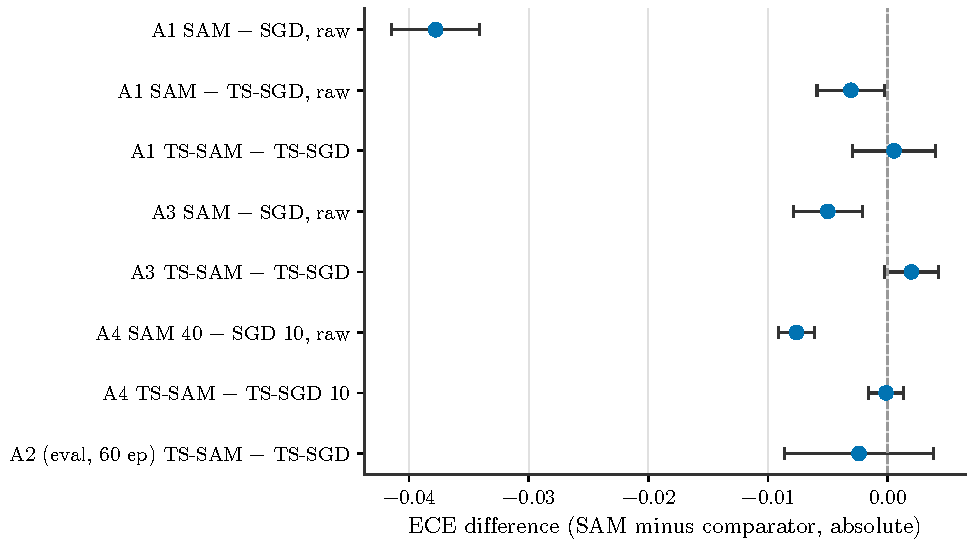
\includegraphics[width=\linewidth,height=0.45\textheight,keepaspectratio]{figures/fig5_v0.pdf}
  \caption{Paired ECE differences, drawn from the same rows as the NLL figure, with the same intervals and the same labels. Raw SAM has lower ECE than raw SGD, but once both models are temperature-scaled, the differences cross zero. Dots are paired-seed means; bars are 95\% t-intervals (five seeds; three for the 60-epoch Artifact 2 row). Negative values favour SAM. The Artifact 3 row for temperature-scaled SAM minus temperature-scaled SGD crosses zero.}
  \label{fig:ece}
\end{figure}

\paragraph{Shuffled-label control.} Table~\ref{tab:placebo} gives the shuffled-label control run in which the test labels are shuffled. Accuracy does not separate the conditions under shuffling (mean difference -0.00032, p = 0.63). NLL and Brier do separate the conditions under shuffling (NLL shuffled-label control difference -0.22405, p = 0.009, Holm p = 0.036). The shuffled-label control therefore does not isolate label information for the proper scoring rules. The artifact reports this as a limitation, and so does this record: the NLL and Brier gaps are not, by themselves, evidence that SAM uses the labels better. The shuffled-label NLL gap of -0.224 is about six times the true-label NLL gap of -0.036 (Table~\ref{tab:primary}).

\begin{table}[!htbp]
\centering
\footnotesize
\caption{Artifact 3 (Iteration 2). Shuffled-label control, test labels shuffled, SAM minus SGD at 40 epochs, five seeds. Read from \texttt{analysis\_tables.json} (shuffled-label control rows).}
\label{tab:placebo}
\begin{tabular}{lrrrr}
\toprule
Contrast & Mean difference & 95\% CI & p (two-sided) & Holm p \\
\midrule
acc & -0.00032 & [-0.00200, +0.00136] & 0.6250 & 0.6250 \\
nll & -0.22405 & [-0.35504, -0.09306] & 0.0090 & 0.0359 \\
ece & +0.00159 & [-0.00058, +0.00376] & 0.1117 & 0.3219 \\
brier & +0.00283 & [+0.00174, +0.00392] & 0.0020 & 0.0099 \\
ace & +0.00160 & [-0.00055, +0.00375] & 0.1073 & 0.3219 \\
PLACEBO SGD minus SGD (same model) & +0.00000 & [+0.00000, +0.00000] & nan & n/a \\
\bottomrule
\end{tabular}
\end{table}

\paragraph{Temperature and training loss.} Table~\ref{tab:cond} gives the per-condition means over the five seeds and the fitted temperatures. The fitted temperature for SGD is above 1, which is the usual overconfidence of a trained network, and the fitted temperature for SAM is below 1, so SAM's confidence falls short of its accuracy on the test set. Both conditions have a final training loss in the same range, about 0.11 to 0.12. The optimiser that fits less is now SGD, which is the reverse of Iteration 1, where SGD reached a training loss of 0.008 and SAM of 0.107. The fit gap therefore depends on the SGD learning rate, not on the optimiser alone.

\begin{table}[!htbp]
\centering
\footnotesize
\caption{Artifact 3 (Iteration 2). Per-condition means over five seeds on the test set, with the fitted temperatures and final training loss. Means are computed from the per-seed records in \texttt{analysis\_tables.json}.}
\label{tab:cond}
\begin{tabular}{lrrrrrrr}
\toprule
Condition & Accuracy & ECE & ACE & NLL & Brier & Mean T & Mean train loss \\
\midrule
SGD, raw & 0.9139 & 0.0125 & 0.0116 & 0.2482 & 0.1269 & 1.049 & 0.1219 \\
SGD, temperature-scaled & 0.9139 & 0.0085 & 0.0076 & 0.2466 & 0.1266 & n/a & n/a \\
SAM, raw & 0.9235 & 0.0075 & 0.0056 & 0.2126 & 0.1111 & 0.938 & 0.1096 \\
SAM, temperature-scaled & 0.9235 & 0.0105 & 0.0089 & 0.2140 & 0.1113 & n/a & n/a \\
\bottomrule
\end{tabular}
\end{table}

\paragraph{Reading.} On the primary family, SAM's accuracy is higher than SGD's by 0.96 points, with an interval of +0.65 to +1.27 points and a Holm p of 0.007. The Iteration 1 accuracy null of +0.15 points was therefore specific to the SGD learning rate of 0.01. Raw ECE is lower for SAM (Holm p = 0.034), and the NLL advantage holds against both raw and temperature-scaled SGD (Holm p = 0.0016 raw, 0.0018 temperature-scaled). The ECE advantage over temperature-scaled SGD is not significant. Its mean is +0.0020 with an interval of -0.0003 to +0.0043, so temperature-scaled SAM is, if anything, slightly worse on ECE. That is the like-for-like result on ECE. In this artifact the rows labelled SAM minus TS-SGD and TS-SAM minus TS-SGD have identical per-seed ECE and NLL differences, so they are one comparison, computed on temperature-scaled SAM. The result matches the like-for-like comparison of Iteration 1 (Table~\ref{tab:cal2}): once both conditions are temperature-scaled, the ECE difference is zero within its interval.

\subsection{Artifact 4: SAM against SGD at matched training loss}

\paragraph{Setup and selection.} Both optimisers use learning rate 0.01, a 0.5 cosine schedule and the same network. The SAM radius 0.1 was chosen on seed 101 by lowest validation NLL, which gave 0.1998 at radius 0.1 against 0.2104 at 0.05 and 0.2299 at 0.2. The matching epoch for SGD was chosen on seed 100. The SAM 40-epoch training loss on that seed was 0.1121. The SGD grid over 10 to 20 epochs gave the first epoch within 0.01 at epoch 10, with a gap of -0.0009, so the matched control is a 10-epoch SGD run at the edge of the grid. Table~\ref{tab:match} gives the matched-loss values per seed and Table~\ref{tab:primA4} gives the primary comparison.

\begin{table}[!htbp]
\centering
\footnotesize
\caption{Artifact 4 (Iteration 2). Matched training loss, per seed. Training losses for SAM at 40 epochs and for SGD at the matched epoch, with the gap between them. Read from \texttt{results/matched\_loss\_table.json}.}
\label{tab:match}
\begin{tabular}{rrrrr}
\toprule
Seed & SAM 40 ep.\ loss & SGD 10 ep.\ loss & Gap & SGD 40 ep.\ loss \\
\midrule
0 & 0.10183 & 0.10497 & +0.00314 & 0.00804 \\
1 & 0.09941 & 0.10439 & +0.00498 & 0.00743 \\
2 & 0.11010 & 0.11120 & +0.00110 & 0.00852 \\
3 & 0.10175 & 0.10723 & +0.00548 & 0.00776 \\
4 & 0.10265 & 0.10302 & +0.00038 & 0.00738 \\
\bottomrule
\end{tabular}
\end{table}

\paragraph{Primary comparison.} Table~\ref{tab:primA4} gives SAM at 40 epochs minus SGD at 10 epochs. The mean differences and intervals are the artifact's stored values. The iteration review recomputed them from the per-run records and found them to agree to the reported digits. The Holm p values are those the artifact's README reports over its fourteen-test family.

\begin{table}[!htbp]
\centering
\footnotesize
\caption{Artifact 4 (Iteration 2). SAM at 40 epochs minus SGD at 10 epochs, five paired seeds, at matched training loss. Mean and 95\% t-interval (df = 4) are the artifact's stored values, recomputed in the iteration review from \texttt{results/runs/}; Holm p is the artifact's value over its fourteen-test family.}
\label{tab:primA4}
\begin{tabular}{lrrrr}
\toprule
Metric & Mean difference & 95\% CI & p (recomputed) & Holm p (README) \\
\midrule
Accuracy & +0.00246 & [+0.00069, +0.00423] & 0.0183 & 0.055 \\
ECE, raw (15 bins) & -0.00761 & [-0.00910, -0.00612] & 0.0001 & 0.0018 \\
ECE, temperature-scaled & -0.00013 & [-0.00159, +0.00134] & 0.8225 & 0.97 \\
NLL, raw & -0.01254 & [-0.01516, -0.00992] & 0.0002 & 0.0019 \\
NLL, temperature-scaled & -0.00818 & [-0.01103, -0.00533] & 0.0013 & 0.0094 \\
Brier, raw & -0.00538 & [-0.00627, -0.00449] & 7.5e-05 & 0.001 \\
ACE, raw & -0.00109 & [-0.00130, -0.00087] & 0.0001 & 0.0018 \\
\bottomrule
\end{tabular}
\end{table}

At matched training loss, the raw ECE and NLL advantages of SAM persist, and so does the NLL advantage after temperature scaling. The temperature-scaled ECE difference is zero within its interval. The accuracy advantage is +0.25 points, with an interval of +0.07 to +0.42 points and a Holm p of 0.055, which the artifact reports as not significant after correction. Matching training loss therefore means the fit gap cannot account for the NLL result in this design. It does not remove the dependence on the SGD learning rate, because the SGD condition here is the weaker baseline described above.

\paragraph{Reference contrast.} Table~\ref{tab:ref4} compares SAM at 40 epochs with SGD at 40 epochs. The SGD condition at 40 epochs reaches a training loss near 0.008, against about 0.10 for SAM and for the matched SGD condition. Its raw ECE is far higher, and its fitted temperature is near 1.9. This pair is the same comparison as Artifact 1 at learning rate 0.01, and it is reported here to show that the matched comparison changes the size of the effect and does not change its direction.

\begin{table}[!htbp]
\centering
\footnotesize
\caption{Artifact 4 (Iteration 2). SAM at 40 epochs minus SGD at 40 epochs, five paired seeds, from \texttt{results/runs/} as stored by the artifact.}
\label{tab:ref4}
\begin{tabular}{lrrr}
\toprule
Metric & Mean difference & 95\% CI & p (two-sided) \\
\midrule
Accuracy & +0.00238 & [-0.00080, +0.00556] & 0.1061 \\
ECE, raw & -0.03726 & [-0.04147, -0.03304] & 1.6e-05 \\
ECE, temperature-scaled & -0.00217 & [-0.00445, +0.00011] & 0.0575 \\
NLL, raw & -0.10086 & [-0.11040, -0.09132] & 8.0e-06 \\
NLL, temperature-scaled & -0.02102 & [-0.02664, -0.01541] & 0.0005 \\
\bottomrule
\end{tabular}
\end{table}

\paragraph{Secondary comparison.} The artifact also compares SAM at 40 epochs with SGD at the epoch of matched loss, read from SGD's own run at that epoch, rather than with a separate 10-epoch run. The artifact's README reports the accuracy difference as +0.0102, the raw ECE difference as -0.0188 and the raw NLL difference as -0.0414, with the temperature-scaled ECE difference as -0.0007 and not significant. These values are the artifact's own summary, and they were not computed again here. The artifact states that models taken before the schedule ends are not final models at a high learning rate, so this comparison is weaker than the primary one and is not used in the reading.


This artifact, \path{gen_art_experiment_4}, matches training loss directly. Its declared output files are \path{method.py}, \path{analysis.py}, \path{audit\_rederive.py}, \path{full_method_out.json}, \path{mini_method_out.json}, \path{preview_method_out.json} and \path{reproducibility.md}; the method output, matched-loss table, tuning record, matched-epoch record, checks and timings are in \path{results/}. The tables below cover its radius selection, its matched-epoch search, its built-in checks, and its re-derivation with a label-permutation placebo.

\begin{table}[!htbp]
\centering
\footnotesize
\caption{Artifact 4 (Iteration 2), gen\_art\_experiment\_4. SAM radius selection on tuning seed 101, read from \texttt{results/tuning.json}. Selection rule: lowest final-epoch validation NLL (raw), test not used. The selected radius is 0.1.}
\label{tab:rho4}
\begin{tabular}{rr}
\toprule
Radius rho & Final validation NLL (seed 101) \\
\midrule
0.05 & 0.21039 \\
0.1 & 0.19984 \\
0.2 & 0.22988 \\
\bottomrule
\end{tabular}
\end{table}
\begin{table}[!htbp]
\centering
\scriptsize
\caption{Artifact 4 (Iteration 2), gen\_art\_experiment\_4. Matched-epoch search for SGD on seed 100, read from \texttt{results/chosen\_E.json}. The reference is SAM's 40-epoch eval-mode training loss on that seed, 0.11208. The rule is the smallest epoch whose training loss is within 0.01 of the reference; epoch 10 was selected, and the grid was not extended.}
\label{tab:matchE4}
\begin{tabular}{rrr}
\toprule
SGD epochs E & SGD training loss & Gap to SAM 40-epoch loss \\
\midrule
10 & 0.11119 & -0.00089 \\
12 & 0.09511 & -0.01696 \\
14 & 0.08011 & -0.03197 \\
16 & 0.06675 & -0.04533 \\
18 & 0.05515 & -0.05693 \\
20 & 0.04587 & -0.06620 \\
\bottomrule
\end{tabular}
\end{table}
\begin{table}[!htbp]
\centering
\scriptsize
\caption{Artifact 4 (Iteration 2), gen\_art\_experiment\_4. Built-in checks of the metric code, the temperature fit, the data split and the SAM implementation at zero radius, read from \texttt{results/checks/checks.json}. Eval-mode logits can differ at rho 0 because batch-norm running statistics are updated in both SAM passes.}
\label{tab:checks4}
\begin{tabular}{lr}
\toprule
Check & Value \\
\midrule
ECE on synthetic perfectly calibrated data (N = 400,000) & 0.00242 \\
ECE on constant confidence 0.8 with accuracy 0.6 & 0.20000 \\
Fitted temperature on synthetic calibrated logits & 0.99552 \\
Logit shape check (batch, classes) & [64, 10] \\
Parameter difference, SAM at rho 0 minus SGD, one epoch & 0.0e+00 \\
Batch-loss difference, SAM at rho 0 minus SGD, one epoch & 0.0e+00 \\
Paired NLL difference, same-seed SGD placebo & 0.0e+00 \\
\bottomrule
\end{tabular}
\end{table}
\begin{table}[!htbp]
\centering
\scriptsize
\caption{Artifact 4 (Iteration 2), gen\_art\_experiment\_4. Independent re-derivation of the primary contrasts from float16 saved logits, read from \texttt{results/audit\_rederivation.json}. The sign-flip p-value is exact; with five seeds its floor is 0.0625.}
\label{tab:audit4}
\begin{tabular}{lrrrrr}
\toprule
Quantity & Re-derived & Stored & Abs.\ diff. & p (t) & p (sign-flip) \\
\midrule
accuracy & +0.00258 & +0.00246 & 1.20e-04 & 0.01687 & 0.0625 \\
ECE, raw & -0.00766 & -0.00761 & 5.14e-05 & 0.0001043 & 0.0625 \\
NLL, raw & -0.01253 & -0.01254 & 3.71e-06 & 0.0001874 & 0.0625 \\
NLL, temperature-scaled & -0.00817 & -0.00818 & 4.54e-06 & 0.001356 & 0.0625 \\
\bottomrule
\end{tabular}
\end{table}
\begin{table}[!htbp]
\centering
\scriptsize
\caption{Artifact 4 (Iteration 2), gen\_art\_experiment\_4. Label-permutation placebo, read from \texttt{results/audit\_rederivation.json}. Accuracy does not reject under permuted labels, while NLL and ECE do, so the placebo gap for NLL and ECE is a confidence effect and not a label effect.}
\label{tab:perm4}
\begin{tabular}{lrrr}
\toprule
Quantity (permuted labels) & Mean difference & p (t) & p (sign-flip, exact) \\
\midrule
accuracy & +0.00024 & 0.5242 & 0.4375 \\
ECE, raw & -0.00708 & 8.464e-06 & 0.0625 \\
NLL, raw & -0.78159 & 6.076e-05 & 0.0625 \\
NLL, temperature-scaled & -0.02768 & 6.405e-05 & 0.0625 \\
\bottomrule
\end{tabular}
\end{table}
\paragraph{Check.} The artifact computed again the primary contrasts from the saved 16-bit logits with separate code. Table~\ref{tab:check4} gives the agreement. The differences are below 1.2e-4, which the artifact attributes to the 16-bit saved logits against 32-bit computation at run time.

\begin{table}[!htbp]
\centering
\footnotesize
\caption{Artifact 4 (Iteration 2). Check of the primary contrasts, SAM at 40 epochs minus SGD at 10 epochs, recomputed from saved logits and compared with the stored values.}
\label{tab:check4}
\begin{tabular}{lrrr}
\toprule
Quantity & Recomputed & Stored & Abs.\ diff. \\
\midrule
accuracy & +0.002580 & +0.002460 & 1.20e-04 \\
ece\_raw & -0.007662 & -0.007610 & 5.14e-05 \\
nll\_raw & -0.012533 & -0.012537 & 3.71e-06 \\
nll\_ts & -0.008173 & -0.008177 & 4.54e-06 \\
\bottomrule
\end{tabular}
\end{table}

\paragraph{Reading.} The matched-loss comparison supports three conclusions at this learning rate: the raw ECE advantage, the raw NLL advantage, and the temperature-scaled NLL advantage, each with an interval that excludes zero. It does not support a temperature-scaled ECE advantage. Five seeds cannot reach an exact p below 0.0625, so none of these results can be significant at 0.05 on an exact test. The t-tests in the tables are parametric and are reported as such.

\subsection{Evaluation 1: the calibration gap across training length}

\paragraph{Setup.} This evaluation reads two existing trajectories and does not pool them. Source 1 is Artifact 1: five paired seeds at 40 epochs, with 5- and 15-epoch compressed schedules, which are separate training runs and not checkpoints of the 40-epoch run. The evaluation also reads Artifact 1's within-run checkpoints at epochs 5 and 15 of the 40-epoch run. Source 2 is Artifact 2: three paired seeds over 60 epochs with per-epoch validation values and a test read at epochs 5 and 60. The two sources use different learning rates (0.01 and 0.03), so their numbers are not comparable across sources.


This evaluation, \path{gen_art_evaluation_1}, trains nothing and recomputes no logits. It reads the declared outputs of Artifact 1 and Artifact 2 and reports the paired gap in each source separately. Its declared output files are \path{eval.py}, \path{full_eval_out.json}, \path{mini_eval_out.json}, \path{preview_eval_out.json} and \path{reproducibility.md}; its gap table, figure specification and caveats are in \path{results/}.

\begin{table}[!htbp]
\centering
\footnotesize
\caption{Evaluation 1 (Iteration 2), gen\_art\_evaluation\_1. The two source trajectories as the evaluation reads them.}
\label{tab:sources5}
\begin{tabular}{p{1.4cm}p{3.6cm}p{1.2cm}p{4.2cm}p{4.6cm}}
\toprule
Source & Artifact read & Seeds & Epochs and learning rate & Validation metrics in the source \\
\midrule
S1 & gen\_art\_experiment\_1 & 5 & 40 (headline); 5 and 15 compressed; learning rate 0.01 & Missing from \texttt{full\_method\_out.json}; recorded as MISSING \\
S2 & gen\_art\_experiment\_2 & 3 & 60; learning rate 0.03 & Present, per epoch \\
\bottomrule
\end{tabular}
\end{table}

The gap table file records the source 1 validation rows as MISSING (n = 0), which is why source 1 carries no validation-ECE or validation-NLL rows in the gap table below. The evaluation's caveats record three design limits: the source 1 shorter lengths are separate schedules, source 1 has no validation metrics, and with three seeds the bootstrap interval is a coarse secondary check only.

\paragraph{Gap table.} The gap table in full follows. It reports the SAM-minus-SGD gap, its t-interval, the raw p-value and the Holm p-value where the artifact computed one, and the per-seed signs. The artifact's bootstrap intervals and notes are in its own \texttt{results/gap\_table.csv}, which is kept with the artifact.

{\scriptsize\setlength{\tabcolsep}{2pt}\begin{longtable}{>{\raggedright\arraybackslash}p{3.6cm}lrrrrrl}
\caption{Evaluation 1 (Iteration 2). Gap table, SAM minus SGD. Source 1 is Artifact 1 and source 2 is Artifact 2. Per-seed signs are written in seed order. Read from \texttt{results/gap\_table.csv}. The ``widening'' rows are differences between two gaps.} \label{tab:gap} \\
\toprule
Comparison (source) & Timepoint & n & Mean gap & 95\% t CI & p (unadj.) & Holm p & Per-seed signs \\
\midrule
\endfirsthead
\toprule
Comparison (source) & Timepoint & n & Mean gap & 95\% t CI & p (unadj.) & Holm p & Per-seed signs \\
\midrule
\endhead
\bottomrule
\endfoot
S1 SAM-SGD test accuracy & epoch 5 (compressed) & 5 & -0.01830 & [-0.02017, -0.01643] & 1.1e-05 & 3.3e-05 & ----- \\
S1 SAM-SGD test accuracy & epoch 15 (compressed) & 5 & -0.00978 & [-0.01234, -0.00722] & 0.0004 & 0.0009 & ----- \\
S1 SAM-SGD test accuracy & epoch 40 (40-epoch run) & 5 & +0.00146 & [-0.00071, +0.00363] & 0.1348 & 0.1348 & -++++ \\
S1 widening: gap(40) minus gap(15), test accuracy & 40 vs 15 & 5 & +0.01124 & [+0.00950, +0.01298] & 5.7e-05 & n/a & +++++ \\
S1 widening: gap(40) minus gap(5), test accuracy & 40 vs 5 & 5 & +0.01976 & [+0.01682, +0.02270] & 4.9e-05 & n/a & +++++ \\
S1 SAM-SGD test ECE & epoch 5 (compressed) & 5 & +0.00574 & [+0.00177, +0.00970] & 0.0159 & 0.0159 & +++++ \\
S1 SAM-SGD test ECE & epoch 15 (compressed) & 5 & -0.01317 & [-0.01625, -0.01009] & 0.0003 & 0.0006 & ----- \\
S1 SAM-SGD test ECE & epoch 40 (40-epoch run) & 5 & -0.03778 & [-0.04145, -0.03412] & 8.8e-06 & 2.6e-05 & ----- \\
S1 widening: gap(40) minus gap(15), test ECE & 40 vs 15 & 5 & -0.02462 & [-0.02861, -0.02062] & 6.8e-05 & n/a & ----- \\
S1 widening: gap(40) minus gap(5), test ECE & 40 vs 5 & 5 & -0.04352 & [-0.04940, -0.03764] & 3.3e-05 & n/a & ----- \\
S1 SAM-SGD test NLL & epoch 5 (compressed) & 5 & +0.04514 & [+0.03915, +0.05113] & 3.1e-05 & 6.2e-05 & +++++ \\
S1 SAM-SGD test NLL & epoch 15 (compressed) & 5 & +0.00650 & [+0.00323, +0.00978] & 0.0053 & 0.0053 & +++++ \\
S1 SAM-SGD test NLL & epoch 40 (40-epoch run) & 5 & -0.09796 & [-0.10918, -0.08673] & 1.7e-05 & 5.2e-05 & ----- \\
S1 widening: gap(40) minus gap(15), test NLL & 40 vs 15 & 5 & -0.10446 & [-0.11323, -0.09570] & 5.0e-06 & n/a & ----- \\
S1 widening: gap(40) minus gap(5), test NLL & 40 vs 5 & 5 & -0.14310 & [-0.15440, -0.13181] & 3.9e-06 & n/a & ----- \\
S1 SAM-SGD test Brier & epoch 5 (compressed) & 5 & +0.02364 & [+0.02096, +0.02632] & 1.7e-05 & 5.0e-05 & +++++ \\
S1 SAM-SGD test Brier & epoch 15 (compressed) & 5 & +0.00920 & [+0.00751, +0.01088] & 0.0001 & 0.0002 & +++++ \\
S1 SAM-SGD test Brier & epoch 40 (40-epoch run) & 5 & -0.01362 & [-0.01792, -0.00933] & 0.0009 & 0.0009 & ----- \\
S1 widening: gap(40) minus gap(15), test Brier & 40 vs 15 & 5 & -0.02282 & [-0.02587, -0.01977] & 3.2e-05 & n/a & ----- \\
S1 widening: gap(40) minus gap(5), test Brier & 40 vs 5 & 5 & -0.03726 & [-0.04153, -0.03299] & 1.7e-05 & n/a & ----- \\
S1 SAM-SGD test ACE & epoch 5 (compressed) & 5 & +0.00665 & [+0.00417, +0.00913] & 0.0017 & 0.0017 & +++++ \\
S1 SAM-SGD test ACE & epoch 15 (compressed) & 5 & -0.01303 & [-0.01635, -0.00971] & 0.0004 & 0.0008 & ----- \\
S1 SAM-SGD test ACE & epoch 40 (40-epoch run) & 5 & -0.03861 & [-0.04282, -0.03440] & 1.4e-05 & 4.2e-05 & ----- \\
S1 widening: gap(40) minus gap(15), test ACE & 40 vs 15 & 5 & -0.02558 & [-0.03047, -0.02070] & 0.0001 & n/a & ----- \\
S1 widening: gap(40) minus gap(5), test ACE & 40 vs 5 & 5 & -0.04527 & [-0.04920, -0.04133] & 5.7e-06 & n/a & ----- \\
S1 SAM-SGD test AURC & epoch 5 (compressed) & 5 & +0.00449 & [+0.00386, +0.00513] & 3.9e-05 & 0.0001 & +++++ \\
S1 SAM-SGD test AURC & epoch 15 (compressed) & 5 & +0.00159 & [+0.00130, +0.00189] & 0.0001 & 0.0002 & +++++ \\
S1 SAM-SGD test AURC & epoch 40 (40-epoch run) & 5 & -0.00152 & [-0.00212, -0.00092] & 0.0021 & 0.0021 & ----- \\
S1 widening: gap(40) minus gap(15), test AURC & 40 vs 15 & 5 & -0.00311 & [-0.00349, -0.00273] & 2.1e-05 & n/a & ----- \\
S1 widening: gap(40) minus gap(5), test AURC & 40 vs 5 & 5 & -0.00601 & [-0.00668, -0.00534] & 1.5e-05 & n/a & ----- \\
S1 SAM-SGD test ECE (within-run checkpoint) & epoch 5 of 40-epoch run & 5 & -0.01333 & [-0.02156, -0.00509] & 0.0109 & n/a & ----- \\
S1 SAM-SGD test ECE (within-run checkpoint) & epoch 15 of 40-epoch run & 5 & -0.02899 & [-0.03561, -0.02238] & 0.0003 & n/a & ----- \\
S1 SAM-SGD test NLL (within-run checkpoint) & epoch 5 of 40-epoch run & 5 & -0.01041 & [-0.02934, +0.00851] & 0.2013 & n/a & --+-- \\
S1 SAM-SGD test NLL (within-run checkpoint) & epoch 15 of 40-epoch run & 5 & -0.04452 & [-0.05455, -0.03449] & 0.0002 & n/a & ----- \\
S1 SAM minus TS-SGD test accuracy & epoch 40 (40-epoch run) & 5 & +0.00146 & [-0.00071, +0.00363] & 0.1348 & n/a & -++++ \\
S1 SAM minus TS-SGD test ECE & epoch 40 (40-epoch run) & 5 & -0.00307 & [-0.00590, -0.00024] & 0.0397 & n/a & ----- \\
S1 SAM minus TS-SGD test NLL & epoch 40 (40-epoch run) & 5 & -0.02088 & [-0.02662, -0.01514] & 0.0005 & n/a & ----- \\
S1 SAM minus TS-SGD test ACE & epoch 40 (40-epoch run) & 5 & -0.00235 & [-0.00606, +0.00135] & 0.1530 & n/a & --+-- \\
S1 SAM minus TS-SGD test Brier & epoch 40 (40-epoch run) & 5 & -0.00494 & [-0.00775, -0.00212] & 0.0082 & n/a & ----- \\
S1 SAM minus TS-SGD test AURC & epoch 40 (40-epoch run) & 5 & -0.00151 & [-0.00209, -0.00093] & 0.0019 & n/a & ----- \\
S2 SAM-SGD val ECE & epoch 1 & 3 & -0.00439 & [-0.02314, +0.01437] & 0.4203 & n/a & -+- \\
S2 SAM-SGD val ECE & epoch 2 & 3 & +0.00387 & [-0.00924, +0.01698] & 0.3320 & n/a & +++ \\
S2 SAM-SGD val ECE & epoch 5 & 3 & +0.00220 & [-0.02829, +0.03270] & 0.7855 & n/a & +-- \\
S2 SAM-SGD val ECE & epoch 10 & 3 & -0.01249 & [-0.02417, -0.00080] & 0.0442 & n/a & --- \\
S2 SAM-SGD val ECE & epoch 15 & 3 & -0.02493 & [-0.03264, -0.01721] & 0.0051 & n/a & --- \\
S2 SAM-SGD val ECE & epoch 20 & 3 & -0.02755 & [-0.02998, -0.02512] & 0.0004 & n/a & --- \\
S2 SAM-SGD val ECE & epoch 25 & 3 & -0.03257 & [-0.04470, -0.02043] & 0.0074 & n/a & --- \\
S2 SAM-SGD val ECE & epoch 30 & 3 & -0.03213 & [-0.03700, -0.02726] & 0.0012 & n/a & --- \\
S2 SAM-SGD val ECE & epoch 35 & 3 & -0.02970 & [-0.03707, -0.02232] & 0.0033 & n/a & --- \\
S2 SAM-SGD val ECE & epoch 40 & 3 & -0.02602 & [-0.02813, -0.02390] & 0.0004 & n/a & --- \\
S2 SAM-SGD val ECE & epoch 45 & 3 & -0.02085 & [-0.02559, -0.01610] & 0.0028 & n/a & --- \\
S2 SAM-SGD val ECE & epoch 50 & 3 & -0.01912 & [-0.02441, -0.01384] & 0.0041 & n/a & --- \\
S2 SAM-SGD val ECE & epoch 55 & 3 & -0.01860 & [-0.02559, -0.01160] & 0.0076 & n/a & --- \\
S2 SAM-SGD val ECE & epoch 60 & 3 & -0.01861 & [-0.02390, -0.01333] & 0.0043 & n/a & --- \\
S2 widening: gap(60) minus gap(1), val ECE & 60 vs 1 & 3 & -0.01423 & [-0.02891, +0.00046] & 0.0530 & n/a & --- \\
S2 widening: gap(60) minus gap(5), val ECE & 60 vs 5 & 3 & -0.02081 & [-0.05415, +0.01252] & 0.1151 & n/a & --- \\
S2 SAM-SGD val NLL & epoch 1 & 3 & +0.03374 & [+0.00118, +0.06629] & 0.0468 & n/a & +++ \\
S2 SAM-SGD val NLL & epoch 2 & 3 & +0.01627 & [+0.01156, +0.02098] & 0.0045 & n/a & +++ \\
S2 SAM-SGD val NLL & epoch 5 & 3 & -0.00073 & [-0.03996, +0.03850] & 0.9435 & n/a & +-- \\
S2 SAM-SGD val NLL & epoch 10 & 3 & -0.00627 & [-0.01848, +0.00594] & 0.1577 & n/a & --- \\
S2 SAM-SGD val NLL & epoch 15 & 3 & -0.04193 & [-0.08781, +0.00395] & 0.0590 & n/a & --- \\
S2 SAM-SGD val NLL & epoch 20 & 3 & -0.05927 & [-0.06191, -0.05664] & 0.0001 & n/a & --- \\
S2 SAM-SGD val NLL & epoch 25 & 3 & -0.08660 & [-0.14196, -0.03125] & 0.0214 & n/a & --- \\
S2 SAM-SGD val NLL & epoch 30 & 3 & -0.09527 & [-0.12979, -0.06074] & 0.0070 & n/a & --- \\
S2 SAM-SGD val NLL & epoch 35 & 3 & -0.09487 & [-0.13568, -0.05406] & 0.0098 & n/a & --- \\
S2 SAM-SGD val NLL & epoch 40 & 3 & -0.08329 & [-0.10923, -0.05734] & 0.0052 & n/a & --- \\
S2 SAM-SGD val NLL & epoch 45 & 3 & -0.07575 & [-0.09514, -0.05636] & 0.0035 & n/a & --- \\
S2 SAM-SGD val NLL & epoch 50 & 3 & -0.07074 & [-0.09756, -0.04392] & 0.0077 & n/a & --- \\
S2 SAM-SGD val NLL & epoch 55 & 3 & -0.06917 & [-0.09720, -0.04115] & 0.0088 & n/a & --- \\
S2 SAM-SGD val NLL & epoch 60 & 3 & -0.06903 & [-0.09532, -0.04274] & 0.0077 & n/a & --- \\
S2 widening: gap(60) minus gap(1), val NLL & 60 vs 1 & 3 & -0.10277 & [-0.13743, -0.06810] & 0.0061 & n/a & --- \\
S2 widening: gap(60) minus gap(5), val NLL & 60 vs 5 & 3 & -0.06830 & [-0.13322, -0.00338] & 0.0455 & n/a & --- \\
S2 val ECE gap vs SGD training loss, per-seed OLS slope & epochs 1-60 (14 logged) & 3 & +0.06531 & [+0.02656, +0.10405] & n/a & n/a & +++ \\
S2 val ECE gap vs SAM training loss, per-seed OLS slope & epochs 1-60 (14 logged) & 3 & +0.05633 & [+0.02643, +0.08623] & n/a & n/a & +++ \\
S2 val NLL gap vs SGD training loss, per-seed OLS slope & epochs 1-60 (14 logged) & 3 & +0.28912 & [+0.18641, +0.39183] & n/a & n/a & +++ \\
S2 val NLL gap vs SAM training loss, per-seed OLS slope & epochs 1-60 (14 logged) & 3 & +0.26532 & [+0.15616, +0.37448] & n/a & n/a & +++ \\
S2 SAM-SGD test accuracy & epoch 5 (test endpoint) & 3 & +0.00123 & [-0.01338, +0.01585] & 0.7513 & n/a & -++ \\
S2 SAM-SGD test ECE & epoch 5 (test endpoint) & 3 & -0.00417 & [-0.02677, +0.01843] & 0.5106 & n/a & +-- \\
S2 SAM-SGD test NLL & epoch 5 (test endpoint) & 3 & -0.00233 & [-0.04064, +0.03598] & 0.8181 & n/a & +-- \\
S2 SAM-SGD test Brier & epoch 5 (test endpoint) & 3 & -0.00194 & [-0.02410, +0.02022] & 0.7422 & n/a & +-- \\
S2 SAM-SGD test ACE & epoch 5 (test endpoint) & 3 & -0.00311 & [-0.02827, +0.02204] & 0.6479 & n/a & +-- \\
S2 SAM raw minus TS-SGD ECE & epoch 5 (test endpoint) & 3 & +0.00132 & [-0.01318, +0.01581] & 0.7331 & n/a & +-+ \\
S2 SAM raw minus TS-SGD NLL & epoch 5 (test endpoint) & 3 & -0.00023 & [-0.03752, +0.03706] & 0.9813 & n/a & +-+ \\
S2 SAM-TS minus SGD-TS ECE & epoch 5 (test endpoint) & 3 & +0.00050 & [-0.00984, +0.01084] & 0.8553 & n/a & +-+ \\
S2 SAM-TS minus SGD-TS NLL & epoch 5 (test endpoint) & 3 & -0.00147 & [-0.03530, +0.03236] & 0.8692 & n/a & +-- \\
S2 SAM-SGD test accuracy & epoch 60 (test endpoint) & 3 & +0.00120 & [-0.00327, +0.00567] & 0.3675 & n/a & +-+ \\
S2 SAM-SGD test ECE & epoch 60 (test endpoint) & 3 & -0.01710 & [-0.02073, -0.01347] & 0.0024 & n/a & --- \\
S2 SAM-SGD test NLL & epoch 60 (test endpoint) & 3 & -0.07613 & [-0.09189, -0.06037] & 0.0023 & n/a & --- \\
S2 SAM-SGD test Brier & epoch 60 (test endpoint) & 3 & -0.01009 & [-0.01474, -0.00543] & 0.0113 & n/a & --- \\
S2 SAM-SGD test ACE & epoch 60 (test endpoint) & 3 & -0.01763 & [-0.02266, -0.01260] & 0.0044 & n/a & --- \\
S2 SAM raw minus TS-SGD ECE & epoch 60 (test endpoint) & 3 & +0.01806 & [+0.01459, +0.02152] & 0.0020 & n/a & +++ \\
S2 SAM raw minus TS-SGD NLL & epoch 60 (test endpoint) & 3 & +0.00342 & [-0.01002, +0.01685] & 0.3880 & n/a & +-+ \\
S2 SAM-TS minus SGD-TS ECE & epoch 60 (test endpoint) & 3 & -0.00239 & [-0.00861, +0.00382] & 0.2395 & n/a & --- \\
S2 SAM-TS minus SGD-TS NLL & epoch 60 (test endpoint) & 3 & -0.01641 & [-0.02987, -0.00294] & 0.0345 & n/a & --- \\
S2 SAM-SGD val ECE, largest mean advantage (extremum over logged epochs) & epoch 25 & 3 & -0.03257 & n/a & n/a & n/a & n/a \\
S2 SAM-SGD val NLL, largest mean advantage (extremum over logged epochs) & epoch 30 & 3 & -0.09527 & n/a & n/a & n/a & n/a \\
\end{longtable}}

\paragraph{Reading of the gap table.} Accuracy shows no difference at 40 epochs in source 1 (+0.00146, interval -0.00071 to +0.00363) and at 60 epochs in source 2 (+0.00120, interval -0.00327 to +0.00567). Source 1's ECE and NLL gaps move from a positive value at 5 epochs in the compressed schedule to a negative value at 40 epochs. That compressed reading is the one the Iteration 1 record gave. The within-run checkpoint reads the opposite sign at 5 epochs. The within-run test ECE gap is -0.01333 (interval -0.02156 to -0.00509) at epoch 5, -0.02899 at epoch 15, and -0.03778 at epoch 40. The compressed schedules therefore do not answer criterion (c). Read along a single trajectory, the gap is already negative at 5 epochs and grows to 40 epochs.

Source 2 is near zero for validation ECE at epochs 1 to 5: -0.00439 at epoch 1, +0.00387 at epoch 2, +0.00220 at epoch 5, all with intervals that include zero. The validation ECE gap reaches its largest mean advantage at epoch 25, -0.03257, and then decreases to -0.01861 at epoch 60. The validation NLL gap follows the same shape, with its largest advantage at epoch 30 (-0.09527). The evaluation's summary describes the NLL gap as near zero over epochs 1 to 5. The gap table shows otherwise at epochs 1 and 2: +0.03374 at epoch 1 (interval +0.00118 to +0.06629, raw p = 0.047) and +0.01627 at epoch 2, with SAM worse on validation NLL early in training. The table is the reading used here.

\begin{figure}[!htbp]
  \centering
  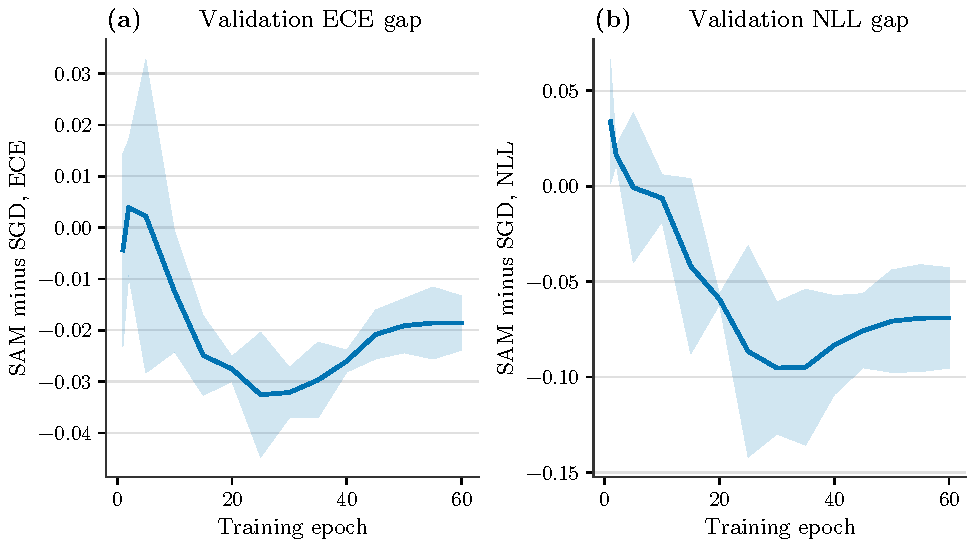
\includegraphics[width=\linewidth,height=0.45\textheight,keepaspectratio]{figures/fig4_v0.pdf}
  \caption{Validation calibration gap, SAM minus SGD, by training epoch (three paired seeds, learning rate 0.03). Values below zero favour SAM. Left: ECE. Right: NLL. Lines are seed means; shaded bands are 95\% t-intervals (df = 2). The bands are wide at early epochs and narrower from about epoch 25 on, and with three seeds the shape of the trajectory is a reading of point estimates only.}
  \label{fig:gap}
\end{figure}

\paragraph{Test endpoints in source 2.} At epoch 60 the test gaps are -0.01710 for ECE (interval -0.02073 to -0.01347) and -0.07613 for NLL (interval -0.09189 to -0.06037). After both models are temperature-scaled, the NLL difference is -0.01641 (interval -0.02987 to -0.00294, raw p = 0.035) and the ECE difference is -0.00239 (interval -0.00861 to +0.00382). Temperature scaling of SGD removes almost all of the ECE gap. The NLL advantage remains, at about a fifth of its raw size, which matches the re-tuned and matched-loss readings below.

\paragraph{Limits of the evaluation.} The evaluation's own caveats hold and are restated here. With three seeds the smallest exact p-value is 0.25, and with five seeds 0.0625, so the parametric p-values in the table are not evidence. The slopes of gap against training loss reflect relationship within one trajectory, not a test of overfitting, because the two conditions reach different training losses at the same epoch. The evaluation's shuffled-label control check rejects only at the smallest attainable p-value of its test.

\subsection{Re-reads of Iteration 1 outputs}

Two Iteration 1 outputs were not reported in the Iteration 1 record. The pooled reliability bins are reported in the Iteration 1 section above. The Artifact 2 loss increase within the perturbation radius is reported here, with no change to the conclusions drawn at the time.

\paragraph{Loss increase and Hessian ratio, Artifact 2.} The artifact's per-epoch record also holds the SAM loss increase within the perturbation radius, which is the loss rise inside the perturbation radius of each SAM step. Table~\ref{tab:hessian} gives it at the epochs of the Iteration 1 per-epoch table, with the top Hessian eigenvalues for both optimisers. The loss increase within the radius is between 0.016 and 0.066 across the logged epochs and falls over training. The ratio of SGD's top Hessian eigenvalue to SAM's varies more than the Iteration 1 record stated. It is 2.7 at epoch 1, 3.35 at epoch 25 and 1.9 at epoch 40.

\begin{table}[!htbp]
\centering
\footnotesize
\caption{Artifact 2 (Iteration 2 re-read). Top Hessian eigenvalue for each optimiser and SAM loss increase within the perturbation radius, mean over three seeds at each logged epoch. Read from \texttt{results/per\_epoch.json}.}
\label{tab:hessian}
\begin{tabular}{rrrrr}
\toprule
Epoch & SGD Hessian & SAM Hessian & Ratio SGD/SAM & SAM loss rise in radius \\
\midrule
1 & 24.95 & 9.18 & 2.72 & 0.0662 \\
2 & 20.69 & 6.80 & 3.04 & 0.0389 \\
5 & 19.09 & 6.21 & 3.07 & 0.0461 \\
10 & 15.72 & 6.60 & 2.38 & 0.0514 \\
15 & 20.58 & 6.33 & 3.25 & 0.0354 \\
20 & 19.19 & 6.94 & 2.76 & 0.0381 \\
25 & 22.82 & 6.82 & 3.35 & 0.0340 \\
30 & 25.02 & 8.01 & 3.12 & 0.0484 \\
40 & 14.55 & 7.50 & 1.94 & 0.0262 \\
50 & 19.88 & 7.43 & 2.68 & 0.0240 \\
60 & 20.20 & 7.13 & 2.83 & 0.0164 \\
\bottomrule
\end{tabular}
\end{table}

\subsection{Reasoning on the criteria after this iteration}

\paragraph{Criterion (a), lower test ECE and NLL than tuned SGD.} NLL is lower for SAM in all three designs: Artifact 1 (-0.098 raw against the Iteration 1 SGD), Artifact 3 (-0.036 raw against the re-tuned SGD, Holm p = 0.0016) and Artifact 4 (-0.013 raw against SGD at matched loss, Holm p = 0.0019). Raw ECE is lower in all three designs as well. The conclusion is supported in direction. Its magnitude depends on the SGD learning rate and on the training-loss match. The conclusion is therefore not stated as a single number, and the fit confound is no longer open for the NLL result at matched loss: that gap does not vanish when SGD is trained to the same loss. The confound is still open for the SGD learning rate, because Artifact 4's baseline is not the validation-selected one.

\paragraph{Criterion (b), NLL advantage after temperature scaling.} The NLL advantage persists after temperature scaling in four readings: Artifact 1 (temperature-scaled SAM minus temperature-scaled SGD, -0.0196, interval excludes zero), Artifact 3 (-0.0326, Holm p = 0.0018), Artifact 4 (-0.0082, Holm p = 0.0094) and Artifact 2 at epoch 60 (-0.0164, raw p = 0.035, three seeds, point estimate). The result is consistent across designs, and its size is between about 0.008 and 0.033 NLL units. Criterion (b) holds in this sense, and the NLL claim is kept at its original size.

\paragraph{Criterion (c), a gap larger at full training than at short training.} Read along single trajectories, the gap grows with training. In Artifact 2 the validation ECE gap is near zero at epochs 1 to 5 and reaches -0.033 at epoch 25. In Artifact 1's within-run checkpoints the test ECE gap grows from -0.013 at epoch 5 to -0.038 at epoch 40. Two caveats limit this reading. Artifact 2's gap decreases after epoch 25 and is no longer largest at the endpoint. Artifact 1's gap is already significantly negative at 5 epochs, so the early gap is near zero in one trajectory and clearly negative in the other. Criterion (c) is therefore supported in part: the gap grows with training in both trajectories up to the point each reaches, and the early-training prediction of a near-zero gap holds in one source only.

\paragraph{Criterion ruled out.} The raw ECE advantage of SAM against temperature-scaled SGD is not supported. In the like-for-like paired comparison the difference is +0.00054 in Artifact 1, +0.0020 in Artifact 3 and -0.0001 in Artifact 4, each with an interval that includes zero. This is the sub-claim the hypothesis stated in advance as a possible failure. It failed, and the record says so.

\paragraph{Accuracy.} SAM's accuracy is higher in all designs, and the size depends on the SGD learning rate: +0.15 points at learning rate 0.01 in Artifact 1 (Holm p = 0.135), +0.96 points at the validation-selected 0.001 in Artifact 3 (Holm p = 0.007), and +0.25 points at matched loss in Artifact 4 (Holm p = 0.055). The Iteration 1 statement that accuracy shows no difference is therefore a statement about one SGD setting, and it is corrected in place below.

\subsection{Corrected like-for-like calibrated comparison}

The Iteration 1 claim of a calibrated ECE advantage was checked like-for-like in this iteration. Table~\ref{tab:cal2} is the paired temperature-scaled comparison that Correction 1 below refers to, as recorded for Artifact 1 in the per-run metrics file.

\begin{table}[!htbp]
\centering
\footnotesize
\caption{Artifact 1 (Iteration 2 re-read). Calibrated comparison, epoch 40, five seeds: temperature-scaled SAM minus temperature-scaled SGD, the artifact's values, recomputed in the iteration review from \texttt{per\_run\_metrics.csv}. Paired t-interval, df = 4.}
\label{tab:cal2}
\begin{tabularx}{\linewidth}{>{\raggedright\arraybackslash}p{2.2cm}>{\raggedright\arraybackslash}X r l r}
\toprule
Metric & Per-seed differences (seeds 0-4) & Mean difference & 95\% CI & p (two-sided) \\
\midrule
ECE & +0.00198, -0.00370, +0.00310, +0.00212, -0.00078 & +0.00054 & [-0.00291, +0.00399] & 0.6845 \\
NLL & -0.01667, -0.02792, -0.01881, -0.01550, -0.01926 & -0.01963 & [-0.02569, -0.01357] & 0.0008 \\
Accuracy & -0.00060, +0.00420, +0.00140, +0.00080, +0.00150 & +0.00146 & [-0.00071, +0.00363] & 0.1348 \\
\bottomrule
\end{tabularx}
\end{table}

\subsection{What was learned in Iteration 2}

Four conclusions are now supported that were not before. The NLL advantage of SAM over SGD holds against temperature-scaled SGD in four readings, and it holds at matched training loss. The raw ECE advantage is a confidence-scale effect: temperature scaling removes it in each design, and the like-for-like ECE comparison shows no difference. The accuracy result depends on the SGD learning rate. The SGD baseline that Iteration 1 used was not the validation optimum, and the grid's lower edge was where its selection fell.

Two conclusions were ruled out or reduced. The ECE sub-claim against temperature-scaled SGD is ruled out in the sense the hypothesis defined. The Iteration 1 reading of the early calibration gap as a reversal is reduced: a within-run read of the same trajectory shows the gap already negative at 5 epochs in Artifact 1.

\paragraph{Failed directions, labelled.}

\begin{enumerate}
\item \emph{The SGD learning rate of 0.01 as the tuned baseline.} Killed by Artifact 3's validation search: validation NLL was 0.273 at 0.01 against 0.214 at 0.001, and the 0.01 setting was the Iteration 1 selection on a three-value grid. The Iteration 1 accuracy null depends on this choice. Artifact 4 uses it as a labelled weaker baseline, and that is recorded as a limitation, not as a finding about SAM.
\item \emph{Lower SAM learning rates at radius 0.1.} Killed by Artifact 3's search: validation NLL was 0.248 at learning rate 0.001 and 0.206 at 0.003, against 0.182 at 0.01. Neither was selected.
\item \emph{Compressed schedules as the test of criterion (c).} Confounded: each compressed run is a separate training run with its own cosine schedule. The within-run checkpoints replace it in Evaluation 1, and the compressed reading is kept in the record as what it is.
\item \emph{Test of overfitting through the gap-against-training-loss slope.} Reported by Evaluation 1 as relationship within one trajectory, not a test. It is not used as evidence for a mechanism.
\end{enumerate}

\paragraph{Caveats that remain.} Artifacts 3 and 4 use five seeds, and the source 2 trajectory of the evaluation uses three, so an exact test cannot reach 0.05 and the parametric p-values are the only tests available. The fit direction changed between designs, so no single fit correction applies. The related-work comparison is partly done (Section~\ref{sec:prior}).

\subsection{Review of Iteration 2 and hypothesis update}

The Iteration 2 review scored the record 5 of 5 and did not block it. The reviewer recomputed Artifact 1's epoch-40 paired contrasts, the compressed-schedule contrasts and the within-run gaps from the per-run file, and Artifact 3's ECE row and Artifact 4's matched-loss gaps, and found them to match the report. The reviewer's main points were: (1) the Iteration 1 prior-work artifact had run and had not been reported, which this record now corrects; (2) the record did not name the nearest published results, and the research artifact's comparison with Tan et al.\ states that the temperature-scaling control this run offers is also in Tan et al.'s ResNet setting, which weakens the claim that the control is new to this run; (3) Artifact 3's shuffled-label NLL gap (-0.224) is about six times the true-label gap (-0.036), and Artifact 4's placebo also fails for NLL, so the NLL claim is stated more strongly than the placebo allows; (4) the matched-loss conclusion rests on a SGD baseline at learning rate 0.01 that the record itself calls the weakest of five, so the statement that the fit gap cannot account for the NLL result is scoped to that baseline.

The reviewer scored soundness at 2 of 5 for the NLL conclusion, and not blocking, because the headline numbers are real and reproducible. The hypothesis update was a deepen move. The NLL lead survives temperature scaling in four readings, and the update kept it as a lead rather than a finding. The ECE sub-claim was withdrawn. The NLL claim was restated as a confidence-sensitive effect whose label specificity is not shown, because the shuffled-label gap is larger than the true gap. The next iteration's experiment is named in the next section.

\subsection{What the next iteration takes from this one}

The open question is whether the NLL advantage holds at matched training loss when the SGD baseline is the validation-selected one. The next iteration should run the matched-loss comparison with SGD at learning rate 0.001, which Artifact 3 selected, and with the matching epoch chosen on the same procedure. It should also add seeds, because five seeds cannot give an exact p-value below 0.0625, and it should read criterion (c) from per-epoch test metrics on a single 40-epoch trajectory rather than from validation values alone. The related-work comparison is partly done, and the nearest-neighbour statement with Tan et al.\ and Morosini et al.\ is still required before any positive claim is written up.

\section{Corrections to previous sections}

These corrections are made in place in the Iteration 1 text and are given here so that the record shows them. Previous sentences were not otherwise changed. Each is marked as a correction where it appears.

\begin{enumerate}
\item \textbf{ECE row against temperature-scaled SGD.} The Iteration 1 row compared uncalibrated SAM with temperature-scaled SGD. Two rows were added beneath it, and the like-for-like comparison is in Table~\ref{tab:cal2}. Its ECE difference is +0.00054 with an interval that includes zero, so the calibrated ECE advantage claimed in Iteration 1 is not supported. The NLL difference of -0.01963 holds.
\item \textbf{Conclusions on criterion (a) and accuracy.} The conclusion on criterion (a) holds in direction, but its magnitude depends on the SGD learning rate and on the fit. The Iteration 1 accuracy null of +0.15 points is specific to SGD at learning rate 0.01, which was the lower edge of Iteration 1's grid. At the validation-selected learning rate of 0.001 the accuracy difference is +0.96 points (Table~\ref{tab:primary}).
\item \textbf{Criterion (c), 5-epoch reversal.} The reversal at 5 epochs came from separately trained compressed schedules. Within one training run the test ECE gap at 5 epochs is -0.0133 (Table~\ref{tab:gap}), which is negative, not positive.
\item \textbf{Table label.} The Iteration 1 table of the independent computation has its label corrected (Table~\ref{tab:check1}).
\item \textbf{Scope of the check, Artifact 1.} The check covers the primary paired contrasts and the two control checks. The ECE binning loop and the ACE, Brier and AURC values were not computed again.
\item \textbf{Hessian ratio.} The Iteration 1 text said the SGD top Hessian eigenvalue is two to three times the SAM value at every evaluated epoch. The ratio is 1.9 at epoch 40 and 3.35 at epoch 25, so the statement is corrected to the range given in Table~\ref{tab:hessian}.
\item \textbf{Loss increase within the radius.} The SAM loss increase inside the perturbation radius, which the per-epoch record also holds, is now reported at every logged epoch in Table~\ref{tab:hessian}.
\item \textbf{Wording, conclusions on the NLL advantage.} A sentence about the NLL advantage is restated as ``the NLL advantage remains against temperature-scaled SGD, with Holm p = 0.0027''.
\item \textbf{Prior-work status.} The Iteration 1 statement that the prior-work check did not run, and that the artifact stage returned no artifact, is withdrawn. The check ran and is recorded in Section~\ref{sec:prior}, with the verification flag described there.
\item \textbf{Reference year, Foret et al.} The reference record gave 2020, the arXiv year. The entry is corrected to ICLR 2021.
\end{enumerate}

\section{What the run has learned so far}

This section covers the run as it is after Iteration 2. Previous sections keep the belief each iteration held at the time, and this section is the current reading of the evidence.

\paragraph{Question.} Does sharpness-aware minimisation improve test accuracy and test calibration over standard SGD for a small CNN on Fashion-MNIST, and is any calibration gain more than a global change in confidence?

\paragraph{Where the evidence lies.}

\begin{enumerate}
\item \emph{NLL.} SAM has a lower test NLL than SGD in every design the run has trained, and the advantage persists under temperature scaling of the SGD baseline. Like-for-like (both conditions temperature-scaled), the NLL difference is -0.0196 in Artifact 1 (Table~\ref{tab:cal2}) and -0.0326 in Artifact 3 (Table~\ref{tab:primary}, Holm p = 0.0018). At matched training loss it is -0.0082 (Table~\ref{tab:primA4}, Holm p = 0.0094). Artifact 2's three-seed trajectory gives -0.0164 at epoch 60, as a point estimate. The NLL advantage is therefore the most consistent result of the run, and its size depends on the SGD learning rate and on the training-length match. The shuffled-label control gives a larger NLL gap than the real comparison, so the advantage is not shown to be label-specific.
\item \emph{ECE.} The raw test ECE of SAM is lower than SGD's in every design (Tables~\ref{tab:primary}, \ref{tab:primA4} and \ref{tab:main}), by between 0.005 and 0.038 depending on the design. The advantage is a global confidence effect. Temperature scaling removes it: the like-for-like ECE differences are +0.00054 (Artifact 1), +0.00199 (Artifact 3) and -0.00013 (Artifact 4), each with an interval that includes zero. The hypothesis's ECE sub-claim is not supported in the form it was stated.
\item \emph{Accuracy.} SAM's accuracy is higher in every design: +0.15 points at SGD learning rate 0.01 (Holm p = 0.135), +0.96 points at the validation-selected SGD learning rate of 0.001 (Holm p = 0.007), and +0.25 points at matched loss (Holm p = 0.055). The size of the accuracy effect is a function of the SGD baseline, and the run does not yet support a single accuracy number.
\item \emph{Training length, criterion (c).} Along single trajectories the calibration gap grows with training. In Artifact 2 the validation ECE gap moves from near zero at epochs 1 to 5 to its largest value at epoch 25 and decreases after that. In Artifact 1's within-run checkpoints the test ECE gap grows from -0.013 at epoch 5 to -0.038 at epoch 40. The early-training prediction of a near-zero gap holds in one source and fails in the other.
\item \emph{Mechanism.} In Artifact 2 SAM's top Hessian eigenvalue is 1.9 to 3.35 times smaller than SGD's across the logged epochs, and the SAM loss increase within the perturbation radius is between 0.016 and 0.066. Matched in training loss, SAM's validation ECE is lower by 0.010 to 0.014, which Artifact 2 reports at three seeds. These are relationships within the runs, not a test of the mechanism.
\end{enumerate}

\paragraph{What the run has changed or reduced.} The Iteration 1 SGD baseline at learning rate 0.01 was not the validation optimum; the lower edge of its grid was the selection. The Iteration 1 claim that accuracy shows no difference, and its calibrated ECE claim, do not hold under the like-for-like and re-tuned comparisons. The Iteration 1 reversal at 5 epochs came from comparing separately trained schedules. The fit gap between the optimisers changes sign between designs: SAM is less fitted at learning rate 0.01 (Artifact 1) and SGD is less fitted at learning rate 0.001 (Artifact 3), so a fit correction cannot be applied as one fixed correction. The prior-work check ran in Iteration 1 and reports the nearest published setting (Tan et al.) as already comparing SAM with temperature-scaled SGD on ResNets at CIFAR scale; this run adds a small CNN on Fashion-MNIST, a temperature-scaled NLL control and a matched-loss comparison.

\paragraph{Hypothesis summary.} The NLL claim is kept, with a size that reflects the SGD baseline and the training-length match, and it is not shown to be label-specific. The ECE sub-claim is not supported. Criterion (c) is supported in part. Criterion (a) holds in direction across designs, and its magnitude is not fixed. Accuracy is recorded as a positive difference whose size depends on the baseline. The run does not yet contain a result that is significant at 0.05 on an exact test, because five seeds set the smallest exact p-value at 0.0625. Every test in the run is parametric.

\paragraph{What remains open.}

\begin{itemize}
\item The nearest-neighbour statement against Tan et al.\ and Morosini et al.\ is not yet written; Morosini et al.\ appear in the reference list but are not cited in the body text of this record.
\item The matched-loss comparison has not been run with the validation-selected SGD learning rate of 0.001.
\item Five seeds are too few for an exact test at 0.05. More seeds are needed before any accuracy or calibration claim is reported as significant.
\item Criterion (c) has not been read from per-epoch test metrics on one trajectory with the validation-selected baseline.
\item The shuffled-label control shows that NLL and Brier respond to shuffled labels, so proper scoring rules do not isolate label information in this design.
\item The 60-epoch extension of Artifact 1 was not run.
\end{itemize}

\subsection*{Run bookkeeping}

The table below is read from the run's trajectory log. Ledger spend is the running total of billed language-model, tool and container spend through each iteration. It excludes compute-rental time, so it is not the run's total cost.

\begin{table}[!htbp]
\centering
\footnotesize
\caption{Run bookkeeping by iteration, from the run's trajectory log. Move is the hypothesis update. Review score is the reviewer's score out of 5. Ledger spend is cumulative through the iteration, in US dollars, and excludes compute-rental time.}
\label{tab:bookkeeping}
\begin{tabularx}{\linewidth}{r l r l l r}
\toprule
Iteration & Move & Review score & Results executed & Evidence state at end & Ledger spend so far (USD) \\
\midrule
1 & deepen & 4 & yes & lead & 0.1530 \\
2 & deepen & 5 & yes & lead & 0.2822 \\
\bottomrule
\end{tabularx}
\end{table}

\section{Code}\label{sec:code}

The code for each experiment artifact is in the paper's code repository, on the run's branch. Each folder below is the one that produced the named results. The prior-work research artifact has no code folder, because it ran web search and PDF extraction only.

\begin{longtable}{>{\raggedright\arraybackslash}p{4.5cm}>{\raggedright\arraybackslash}p{5.2cm}>{\raggedright\arraybackslash}p{4.5cm}}
\toprule
Artifact (iteration) & Result & Code folder \\
\midrule
\endhead
Artifact 1 (Iteration 1) & Controlled comparison, Tables~\ref{tab:tune1}--\ref{tab:check1}, Figure~\ref{fig:paired} & \href{https://github.com/ai-inventor-papers/ai-invention-d46016-sharpness-aware-training-makes-small/tree/main/round-1/experiment-1}{\texttt{round-1/experiment-1}} \\
Artifact 2 (Iteration 1) & Mechanism study, Tables~\ref{tab:perseedA}--\ref{tab:stats2}, Figure~\ref{fig:epoch60} & \href{https://github.com/ai-inventor-papers/ai-invention-d46016-sharpness-aware-training-makes-small/tree/main/round-1/experiment-2}{\texttt{round-1/experiment-2}} \\
Artifact 3 (Iteration 2) & Primary comparison at tuned learning rates, Tables~\ref{tab:tune2}--\ref{tab:cond}, Figures~\ref{fig:nll} and \ref{fig:ece} & \href{https://github.com/ai-inventor-papers/ai-invention-d46016-sharpness-aware-training-makes-small/tree/main/round-2/experiment-3}{\texttt{round-2/experiment-3}} \\
Artifact 4 (Iteration 2) & Matched training loss, Tables~\ref{tab:match}--\ref{tab:check4} & \href{https://github.com/ai-inventor-papers/ai-invention-d46016-sharpness-aware-training-makes-small/tree/main/round-2/experiment-4}{\texttt{round-2/experiment-4}} \\
Evaluation 1 (Iteration 2) & Calibration gap across training length, Table~\ref{tab:gap}, Figure~\ref{fig:gap} & \href{https://github.com/ai-inventor-papers/ai-invention-d46016-sharpness-aware-training-makes-small/tree/main/round-2/evaluation-1}{\texttt{round-2/evaluation-1}} \\
\bottomrule
\end{longtable}

The output files named in this report are kept with each artifact on the run's volume and are not in the published repository. Model checkpoints and per-sample logits are in the artifact folders on the run's volume.

\section*{References}

\begin{thebibliography}{9}
\bibitem[Foret et~al., 2021]{foret2021} P.~Foret, A.~Kleiner, H.~Mobahi, B.~Neyshabur. Sharpness-Aware Minimization for Efficiently Improving Generalization. ICLR 2021. arXiv:2010.01412.
\bibitem[Guo et~al., 2017]{guo2017} C.~Guo, G.~Pleiss, Y.~Sun, K.~Q.~Weinberger. On Calibration of Modern Neural Networks. ICML 2017. arXiv:1706.04599.
\bibitem[Nixon et~al., 2019]{nixon2019} J.~Nixon, M.~W.~Dusenberry, L.~Zhang, G.~Jerfel, D.~Tran. Measuring Calibration in Deep Learning. CVPR Workshops 2019, pp.~38--41. arXiv:1904.01685.
\bibitem[Tan et~al., 2026]{tan2026} C.~Tan, Y.~Zhou, H.~Ye, G.~Dai, J.~Liu, Z.~Song, J.~Zhang, Z.~Zhao, Y.~Hao, Y.~Xu. Towards Understanding The Calibration Benefits of Sharpness-Aware Minimization. ICLR 2026. arXiv:2505.23866.
\bibitem[Morosini et~al., 2026]{morosini2026} A.~Morosini, M.~Gjika, T.~Poggio, P.~Beneventano. Too Sharp, Too Sure: When Calibration Follows Curvature. 2026. arXiv:2604.20614.
\bibitem[M\"uller et~al., 2019]{muller2019} R.~M\"uller, S.~Kornblith, G.~Hinton. When Does Label Smoothing Help? 2019. arXiv:1906.02629.
\bibitem[Xiao et~al., 2017]{xiao2017} H.~Xiao, K.~Rasul, R.~Vollgraf. Fashion-MNIST: a Novel Image Dataset for Benchmarking Machine Learning Algorithms. 2017. arXiv:1708.07747.
\end{thebibliography}

\end{document}
